\documentclass{article}
\usepackage{amsmath}
\usepackage{graphicx}
\begin{document}
\title{Determinants of Wage in East and West Germany}
\author{Christian Koopmann}
\maketitle


\section{Introduction}
Since the fall of the iron curtain the labour markets of countries transitioning from communist to market economies have been the topic of numerous studies and intense discussion in the field of labour economics. One aspect of particular interest in this field of research has been the change of returns to education and experience during this transition. The abruptness of the political change and the existence of a benchmark economy with the same institutional framework let the territory of the former German Democratic Republic stand out among other transitional economies in Europe and Asia. This uniqueness has led to East Germany being the focus of a large number of studies concerning labour market dynamics. 

Two questions of particular interest that will form the focus of this study are: 
\textit{How much value do education and experience obtained in the GDR retain post-unification?} and \textit{How quickly do wage setting regimes in West- and East-Germany converge?}.
The second question has been analysed for varying time frames and methodological approaches. Early analyses were focused on labour markets before and after reunification. These studies have shown much flatter wage profiles across age  (\cite{krueger_comparative_1992},\cite{burda_getting_1997}) as well as experience (\cite{jurajda_when_2007}). \cite{orlowski_east_2009} shows that even after extending the analysis well into the twenty-first century and applying non-OLS estimators to account for endogeneity these differences persist. Two frequently encountered explanations of these results are the presumed low quality of human capital obtained in the GDR as well as continuing differences in regional prices of human capital in east and west Germany. One approach to differentiate between these effects is to divide experience and education into parts that were obtained pre- and post-unification and estimating their returns seperately. This approach has been applied by \cite{gathmann_understanding_2004} and shown pre-unification work experience to be virtually worthless in the post-unification labour market. Since the work experience of older East German employees fall disproportionally into this category, this result offers new insights into the observed difference in lifecycle wage profiles. This paper will use this approach to estimate returns to pre-/post-unification work experience and education in both east and west Germany over the time from 1990 to 2014. To see how the ability to accumulate human capital differs with age and qualification, this analysis will be done seperately for different wage and skill-groups.
\section{Data and Descriptive Evidence}
Similar to most of the papers cited above I will make use of the data of the German Socio-Economic Panel (GSOEP) which is a large scale panel datasets that starts in 1984 for West Germany and 1990 for East Germany. Although the first East German sample was taken after reunification, the retrospective questions allow insights into the economic situation of respondents immediately before reunification. The main basis of this analysis are formed by the \textit{pgenl} and ppfadl datasets  from the \textit{SOEPLong} data, which contains a variety of generated variables (such as years of education) in convenient format for analysis. For further details see \cite{wagner_german_2007}.
The analysis will be limited to full time employed individuals. Whereas the descriptive analysis in this section is based on all representative samples (excluding e.g. the high income sample) the modelling in later sections will be limited to such individuals for which work experience pre- and post-unification can be determined under reasonable assumptions. This encompasses mainly those individuals that entered the study in 1990 or earlier (samples A and C) as well as mainly younger individuals in later samples where pre-unification work experience can be assumed to be zero. The target variables is the hourly wage defined as gross wage divided by actual hours worked deflated to 2010 prices using the Consumer Price Index of the Federal Statistics Office. A first impression of dynamics of the income distribution can be gained by looking at Mean hourly wages in East- and West-Germany as a function of time. Figure \ref{fig:MeanHourlyWagesByAgeGroup} plots this information for different age groups. The graph confirms results of previous studies showing a flat income distribution across age in East-Germany immediately after reunification. In the first years following reunification East German wages have  started to converge with West German levels, a process that has considerably slowed since the mid nineties.
Figure \ref{fig:MeanHourlyWagesBySkillGroup} shows similar results when analysing the data across different skill groups (defined by highest degree obtained). Both graphs however show significantly lower wages in East Germany even 25 years after reunification. Figure \ref{fig:MeanWageDifferentialsBySkillGroup} show that wages of individuals without vocational degree converge significantly slower than those of more highly qualified workers. Figures \ref{fig:RelHourlyWagesByAgeGroup} and \ref{fig:RelHourlyWagesBySkillGroup} which plot mean wages across age and skill groups as multiple of the reference group we get two very different results. The East German wage distribution across age has started out at much flatter levels and slowly converged towards that of West Germany. Regarding skill levels however the East German wage structure has started out fairly similar to that of the west but then diverged from it up until the earl 2000s when it started to return back to the fairly constant distribution in the west. Overall East German workers without vocational degree seemed to have been mostly left out of the  large wage gains in the 1990s and only in the last ten years started to make up some of that ground.
To properly evaluate the results of the next section it is also useful to compare the distribution of the Age and Skill-Group variables itself in the East- and West-German samples. 
Figures \ref{fig:AgeMeans} and \ref{fig:AgeProps} illustrate the ageing process of the panel population (slowed by the inclusion of newer samples) and show that the age distribution seems to be relatively similar in East- and West Germany. Figure \ref{fig:SkillProps} however shows a significant  lower share of college educated workers in the West German sample which linearly rises to East German levels. 
The main focus of this analysis are returns to experience gathered before and after reunification. A first impression of what to expect from this analysis can be gained by grouping the data according to experience and analysing mean wages across these groups.
\bibliographystyle{apalike}. While figures  \ref{fig:MeanHourlyWagesByExpGroup} and \ref{fig:RelHourlyWagesByExpGroup} suggest similar results as we obtained for age groups the picture changes when one differentiates between new and old experience. Figure \ref{fig:RelHourlyWagesByOldExpGroup} shows that old experience in West Germany seems to start off with a relative high value immediately after reunification but then quickly falls to similar levels as in East Germany where the wage distribution across Old Experience is quite flat throughout the time frame. The analysis seems to support the hypothesis that experience obtained in the former GDR is of low value and that the convergence in the experience profile is due to the rising share of new experience.

\section{Determinants of Wage}


\bibliography{EconometricProject}
\begin{figure}[!h]
    \centering
    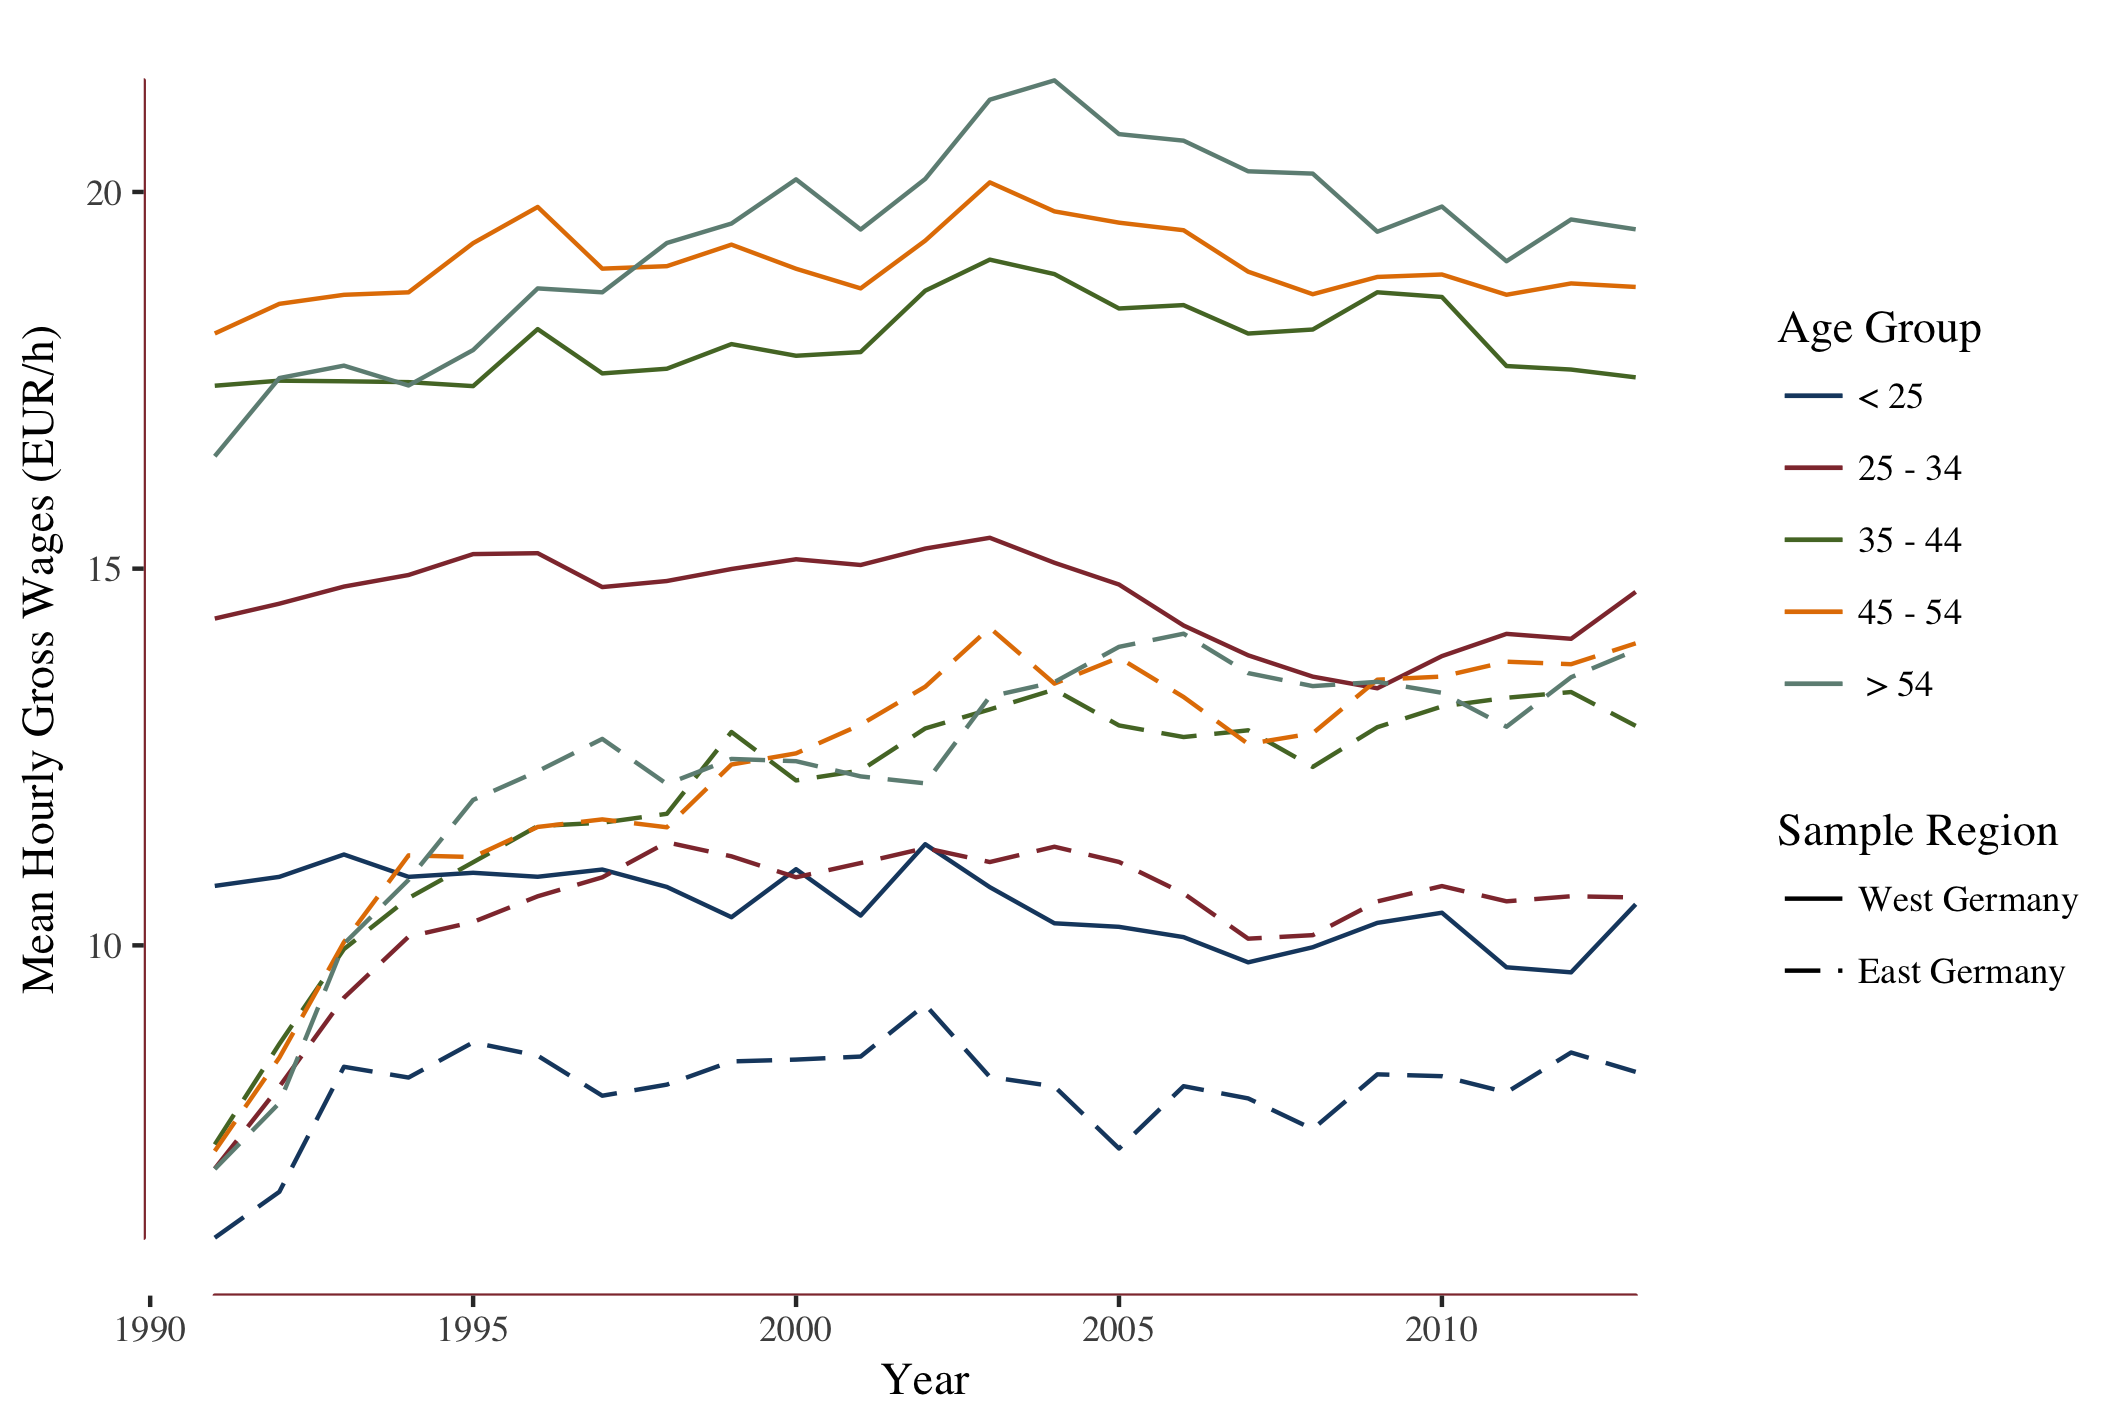
\includegraphics[width=\textwidth]{/Users/Christian/Statistik_Studium/EconProject/Code/Graphics/plotMeanHourlyWagesByAgeGroup.png}
    \caption{Average Hourly Wages in 2010 Euros by Age Group and Sample Region}
    \label{fig:MeanHourlyWagesByAgeGroup}
\end{figure}

\begin{figure}[!h]
    \centering
    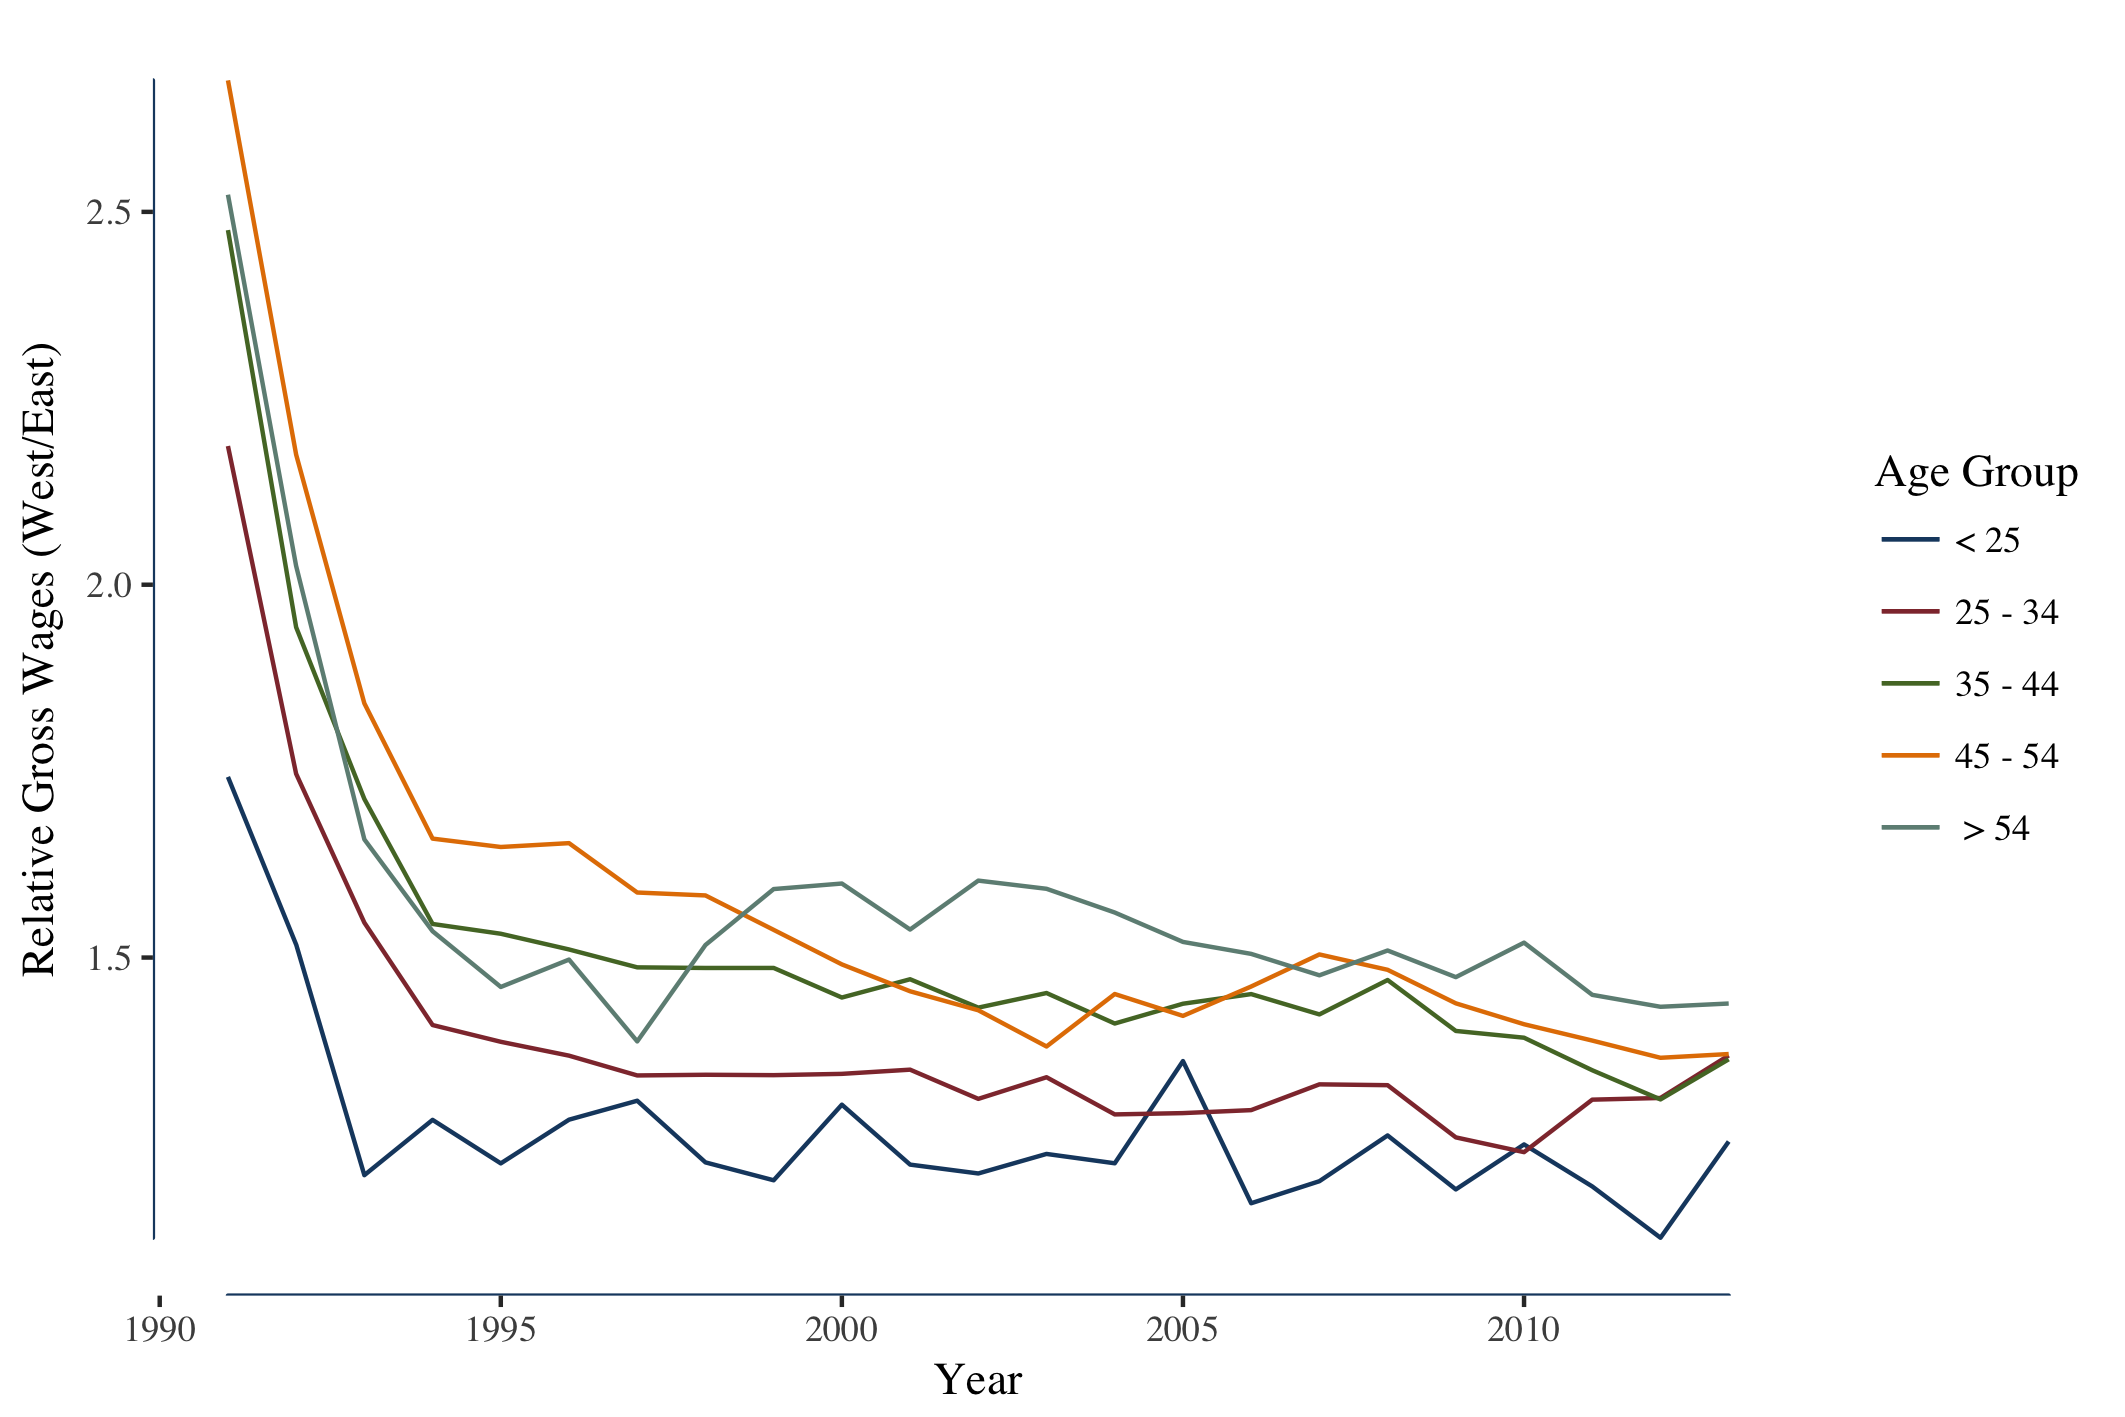
\includegraphics[width=\textwidth]{/Users/Christian/Statistik_Studium/EconProject/Code/Graphics/plotMeanWageDifferentialsByAgeGroup.png}
    \caption{Relative Ages West/East by Age Group}
    \label{fig:MeanWageDifferentialsByAgeGroup}
\end{figure}

\begin{figure}[!h]
    \centering
    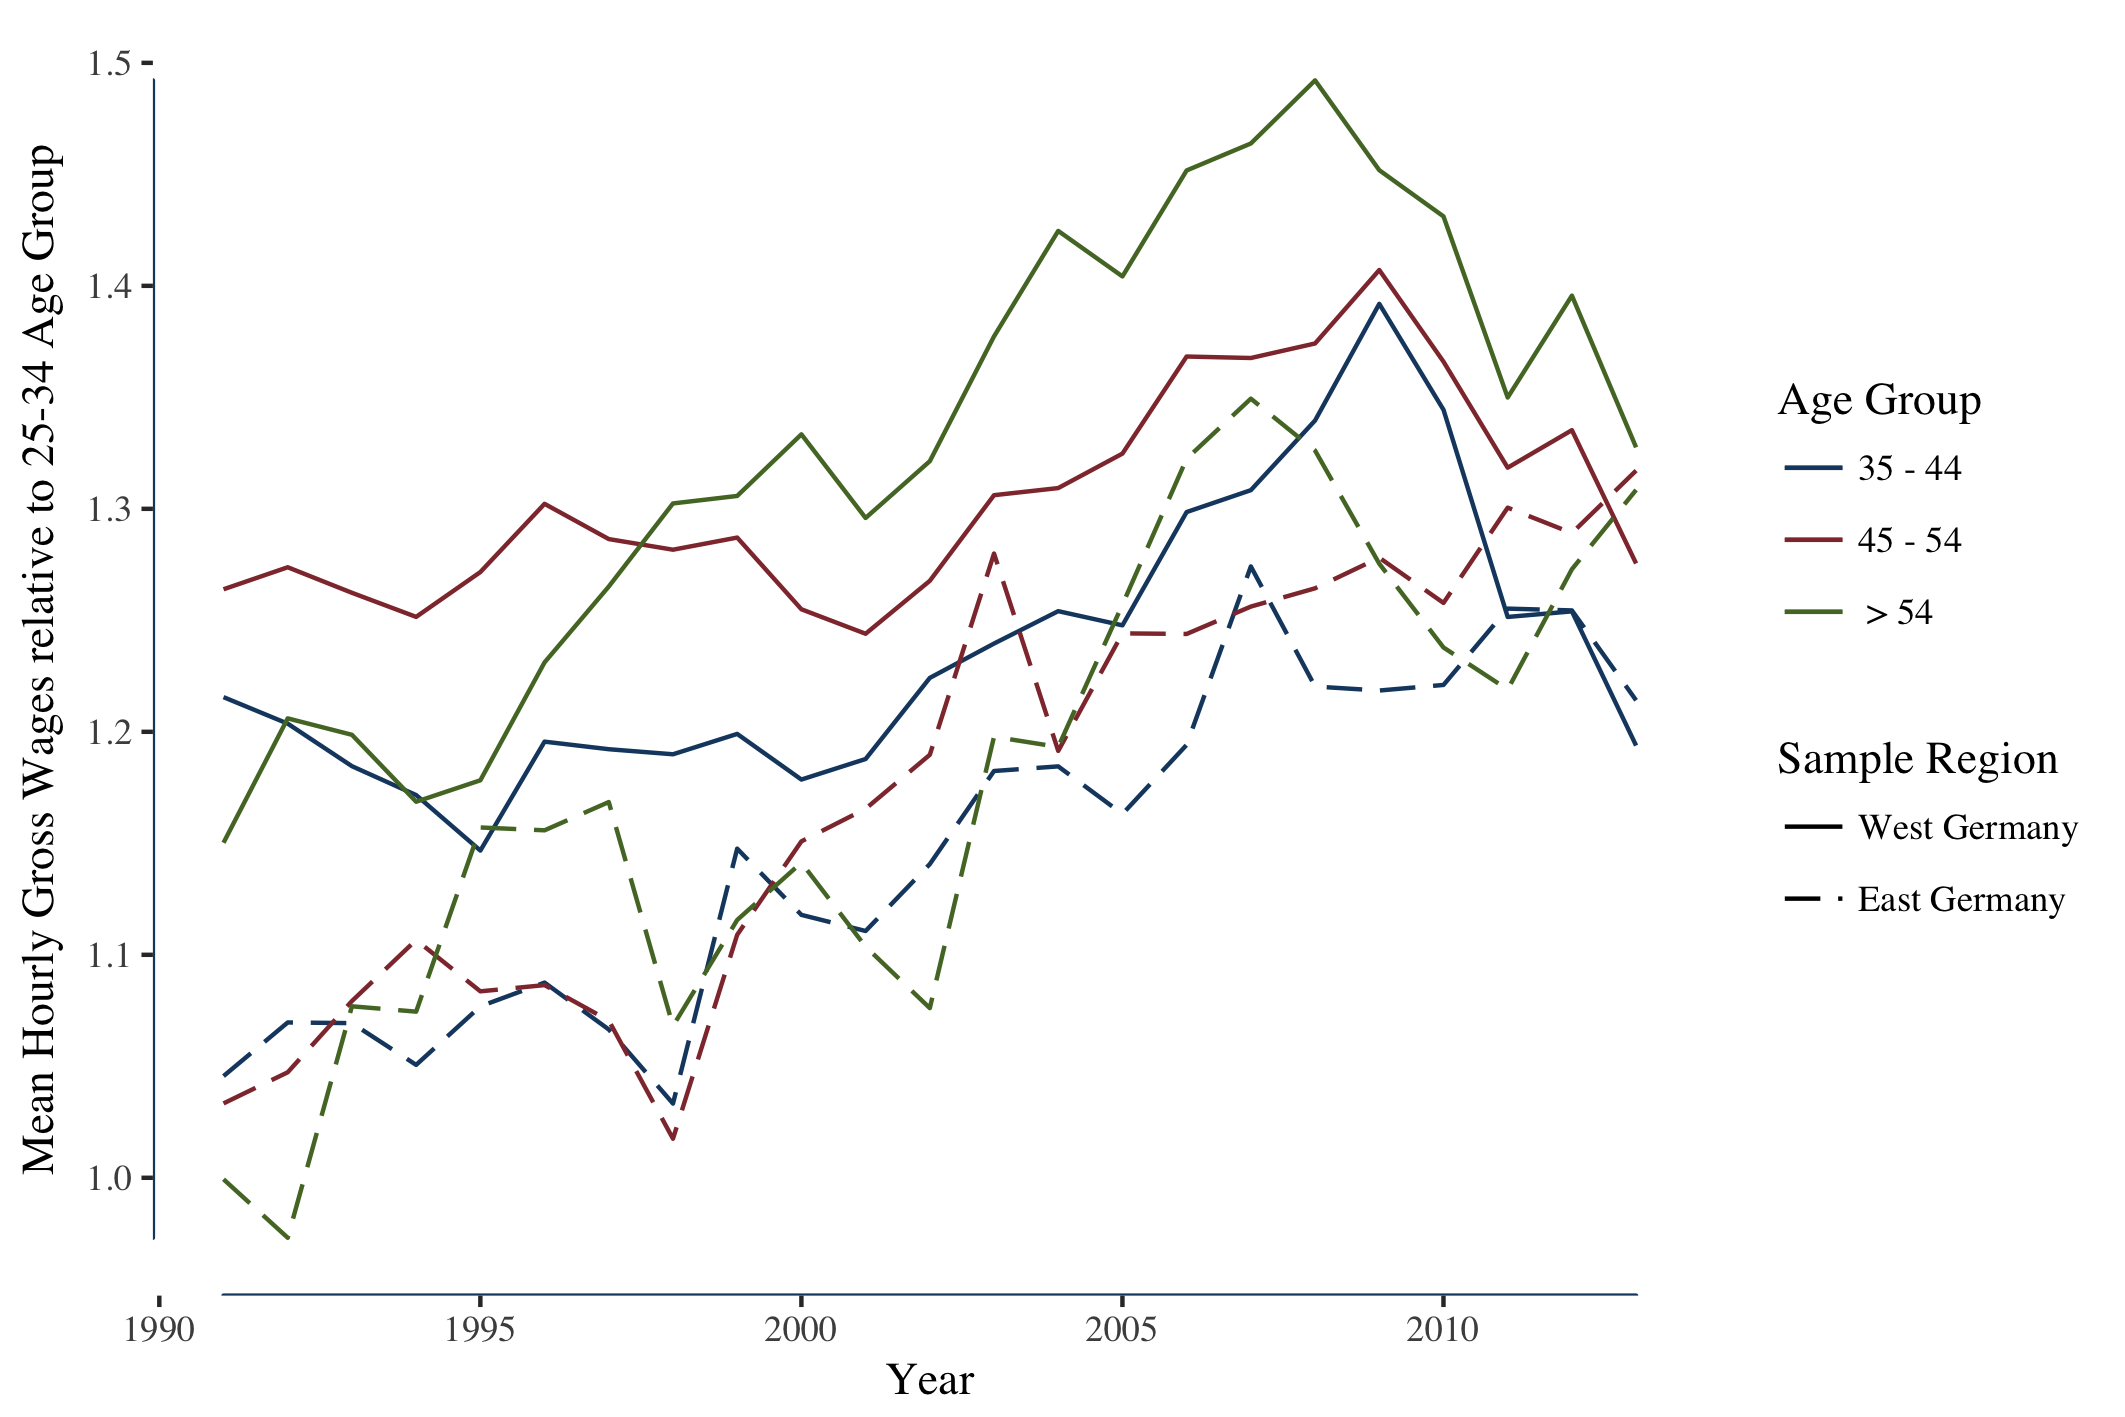
\includegraphics[width=\textwidth]{/Users/Christian/Statistik_Studium/EconProject/Code/Graphics/plotRelHourlyWagesByAgeGroup.png}
    \caption{Relative mean wages across age groups as multiple of mean wage of 25-34 age group.}
    \label{fig:RelHourlyWagesByAgeGroup}
\end{figure}

\begin{figure}[!h]
    \centering
    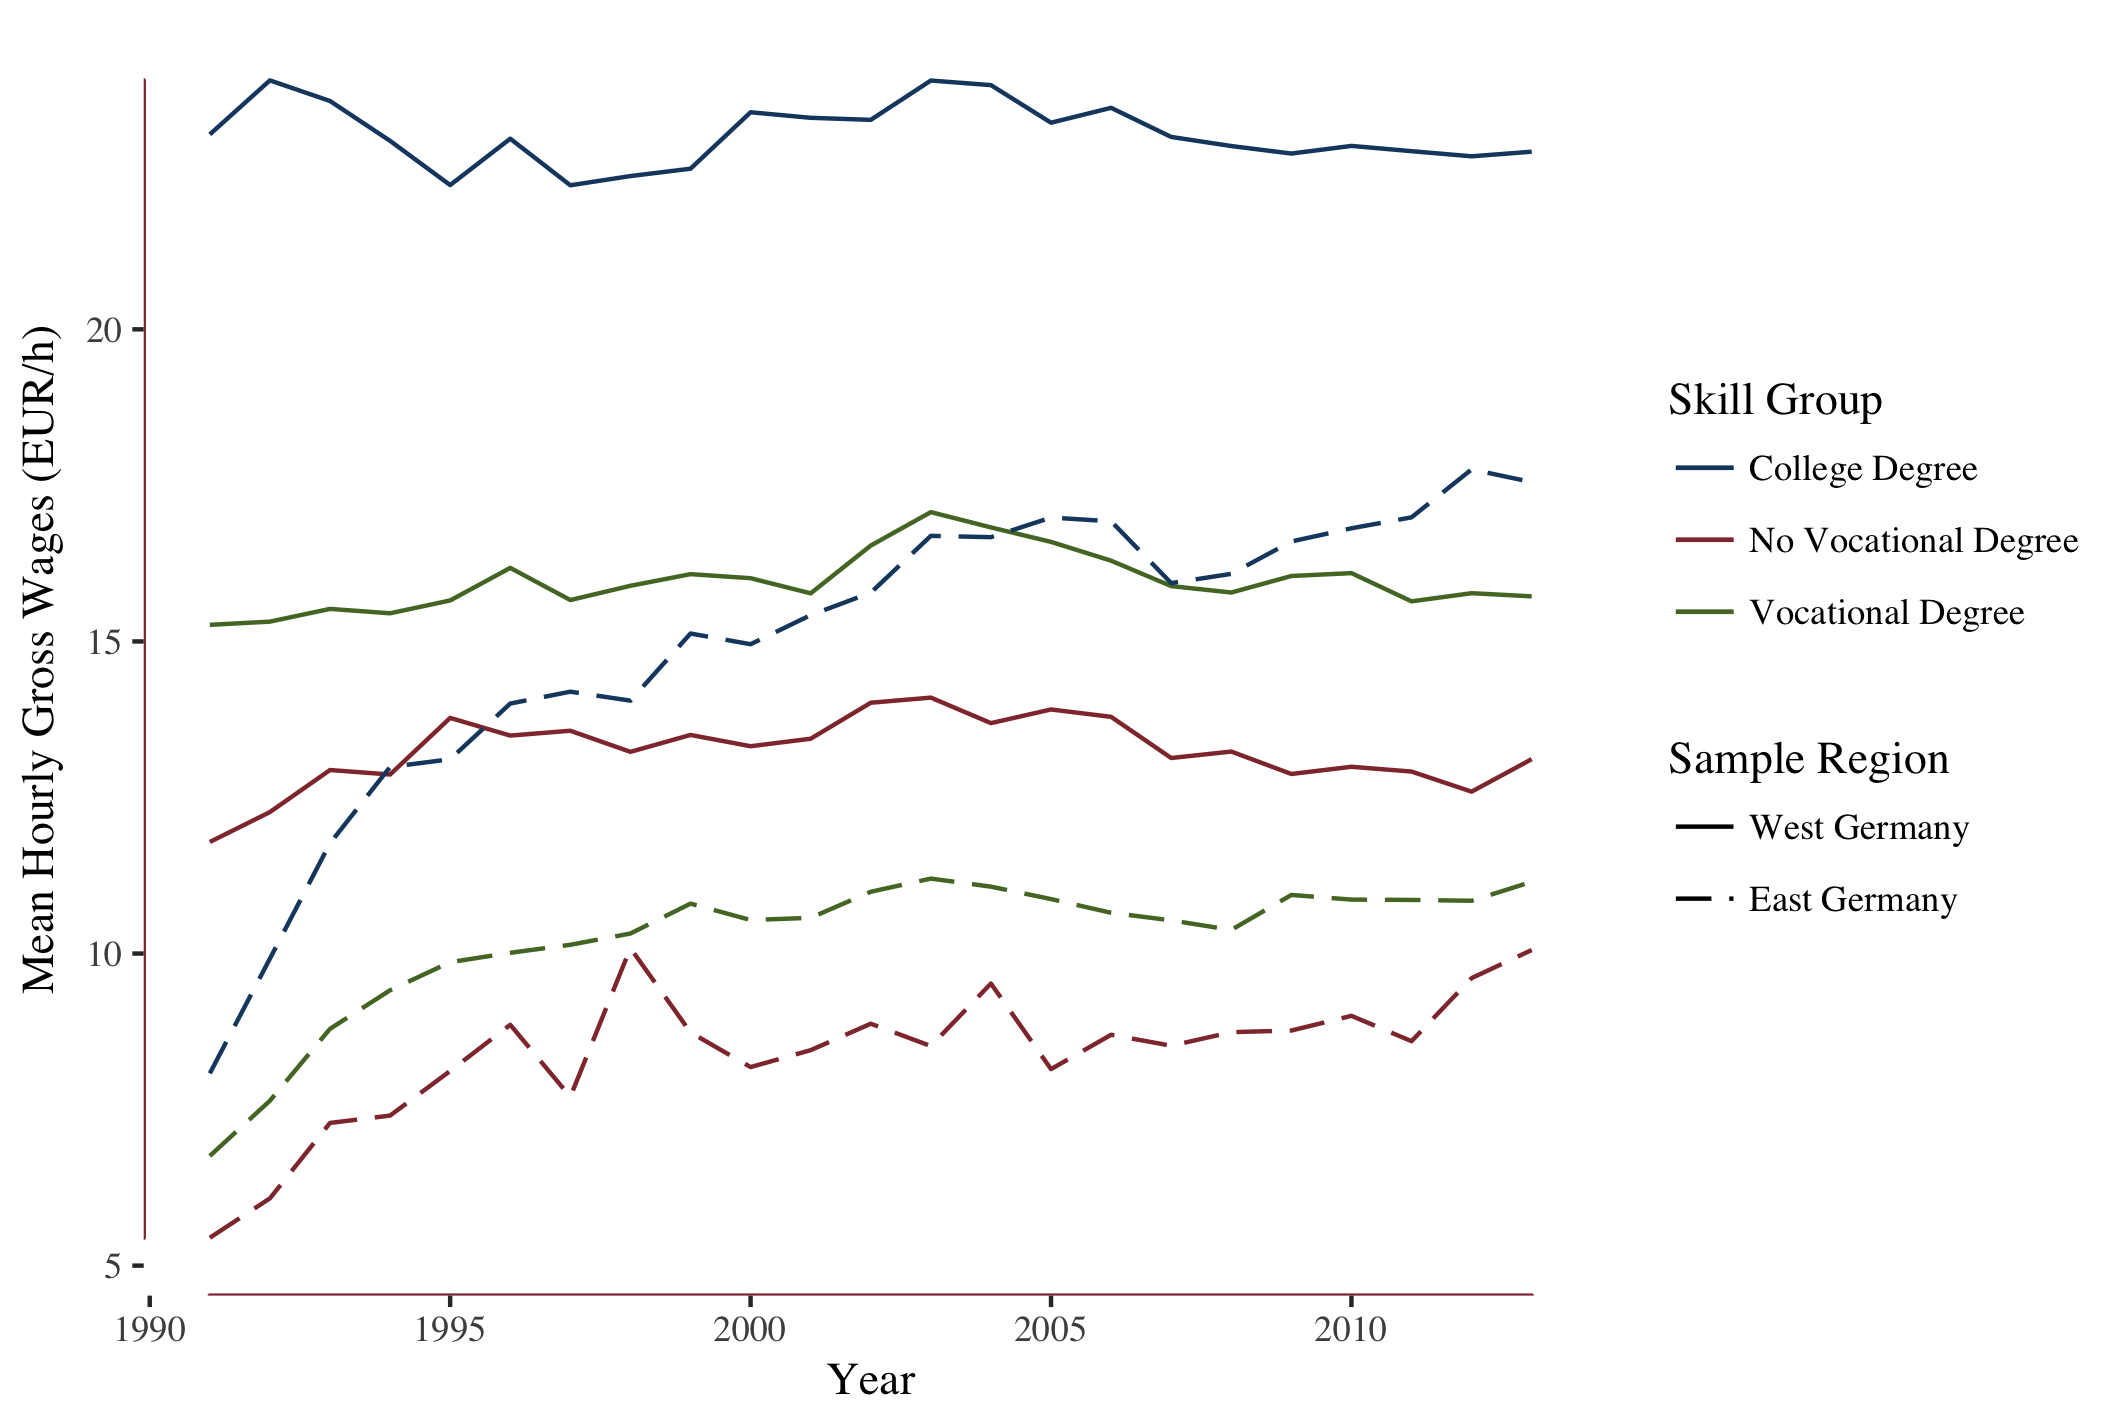
\includegraphics[width=\textwidth]{/Users/Christian/Statistik_Studium/EconProject/Code/Graphics/plotMeanHourlyWagesBySkillGroup.png}
    \caption{Average Hourly Wages in 2010 Euros by Skill Group and Sample Region}
    \label{fig:MeanHourlyWagesBySkillGroup}
\end{figure}

\begin{figure}[!h]
    \centering
    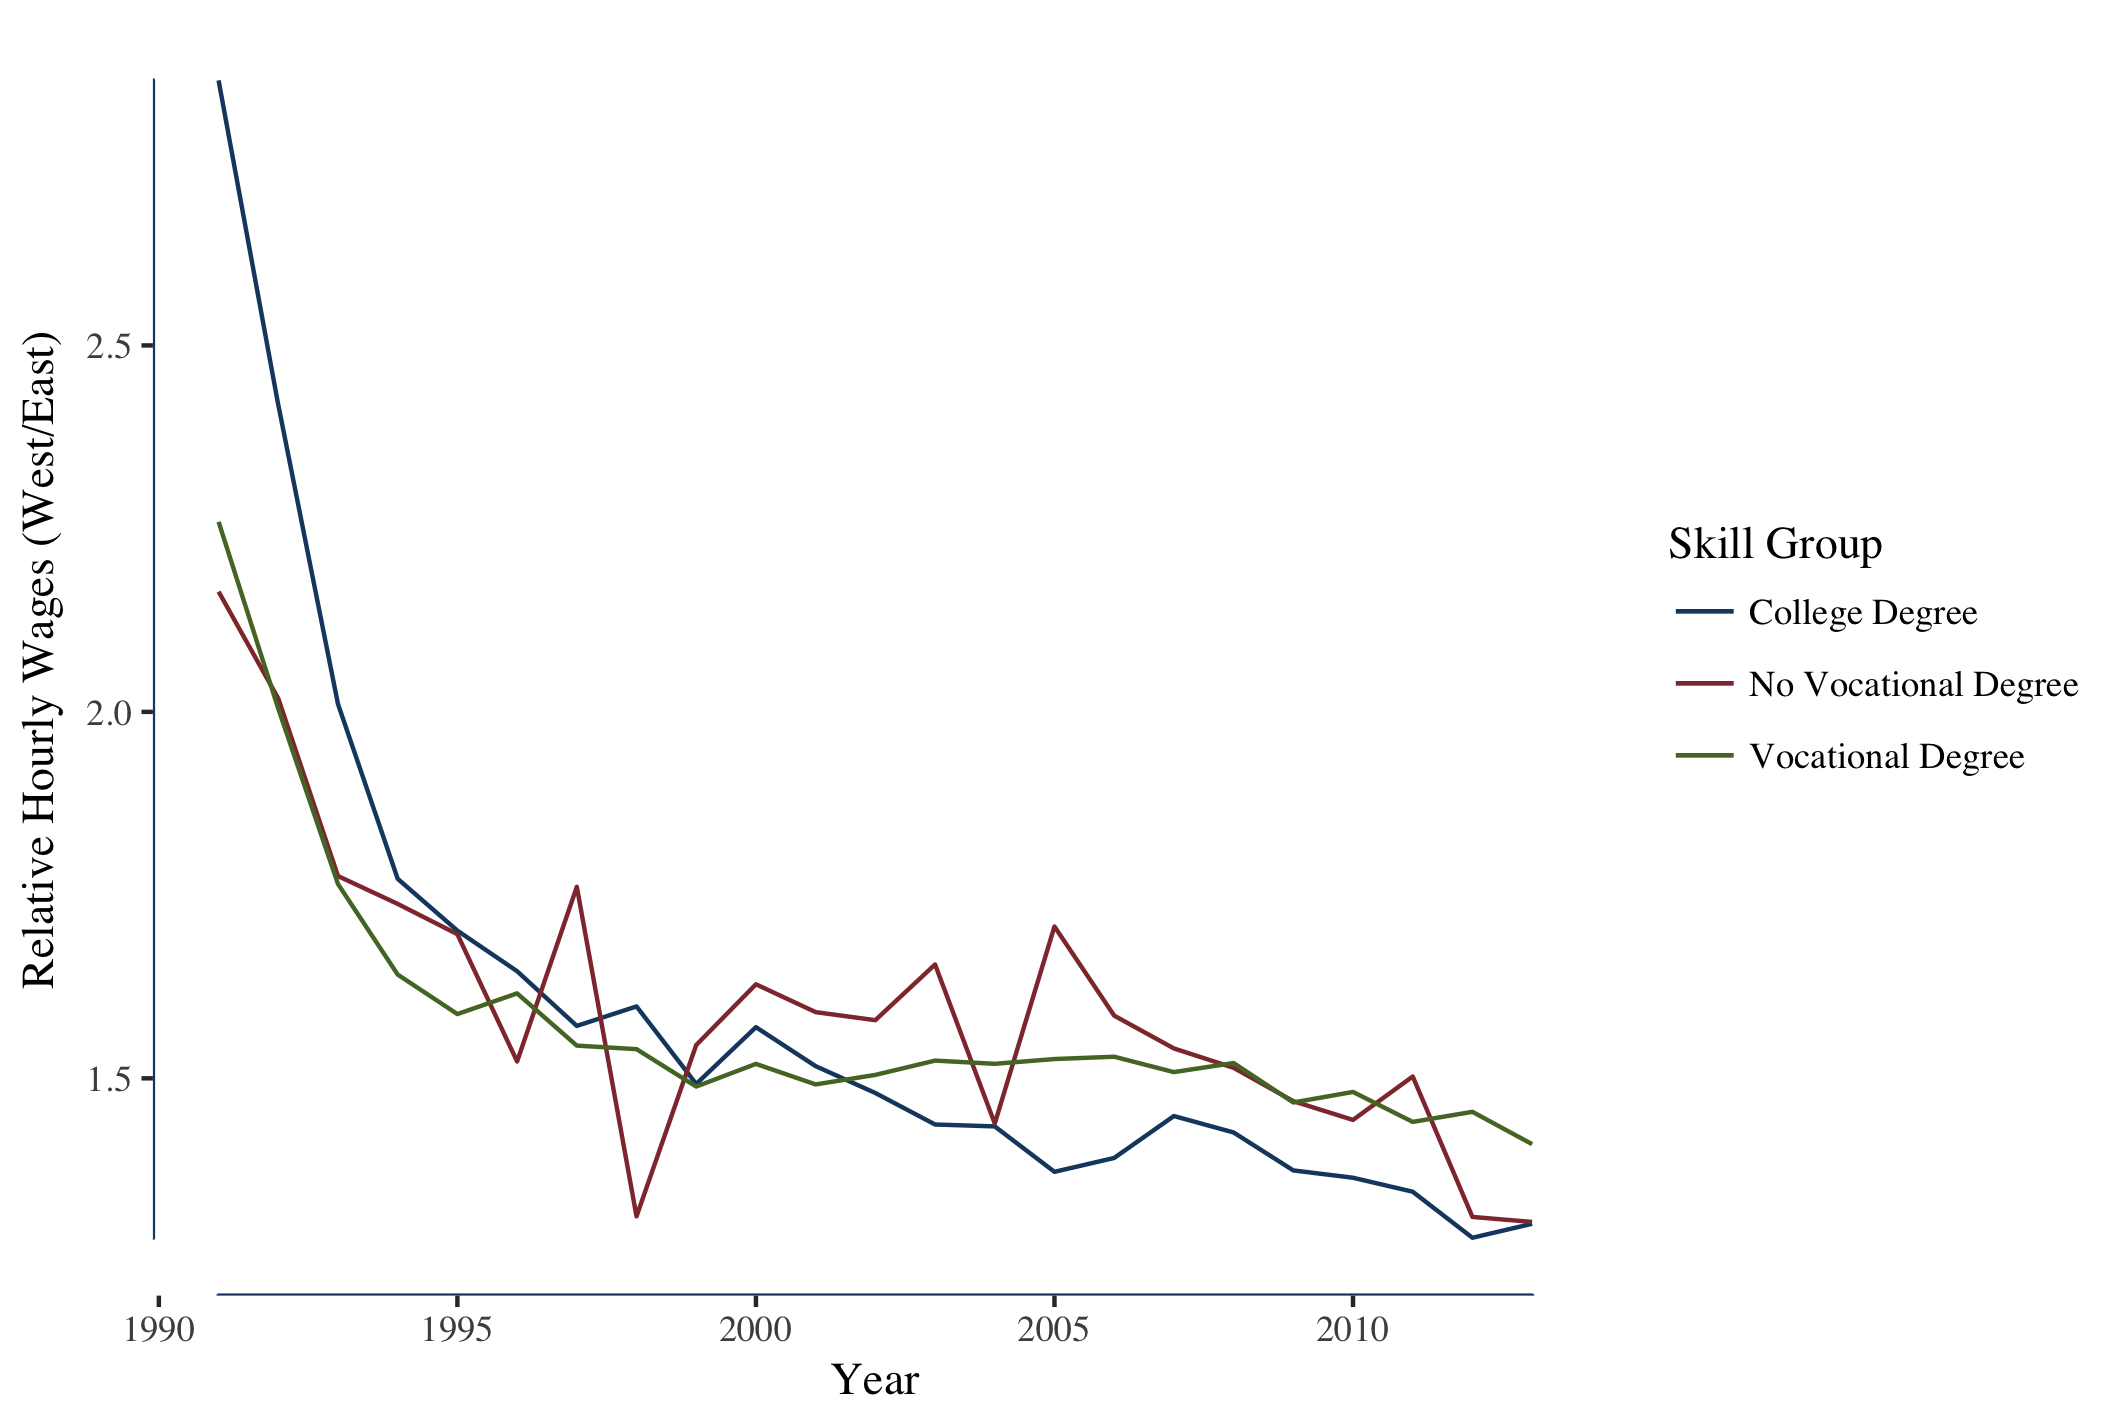
\includegraphics[width=\textwidth]{/Users/Christian/Statistik_Studium/EconProject/Code/Graphics/plotMeanWageDifferentialsBySkillGroup.png}
    \caption{Relative Ages West/East by Skill Group}
    \label{fig:MeanWageDifferentialsBySkillGroup}
\end{figure}

\begin{figure}[!h]
    \centering
    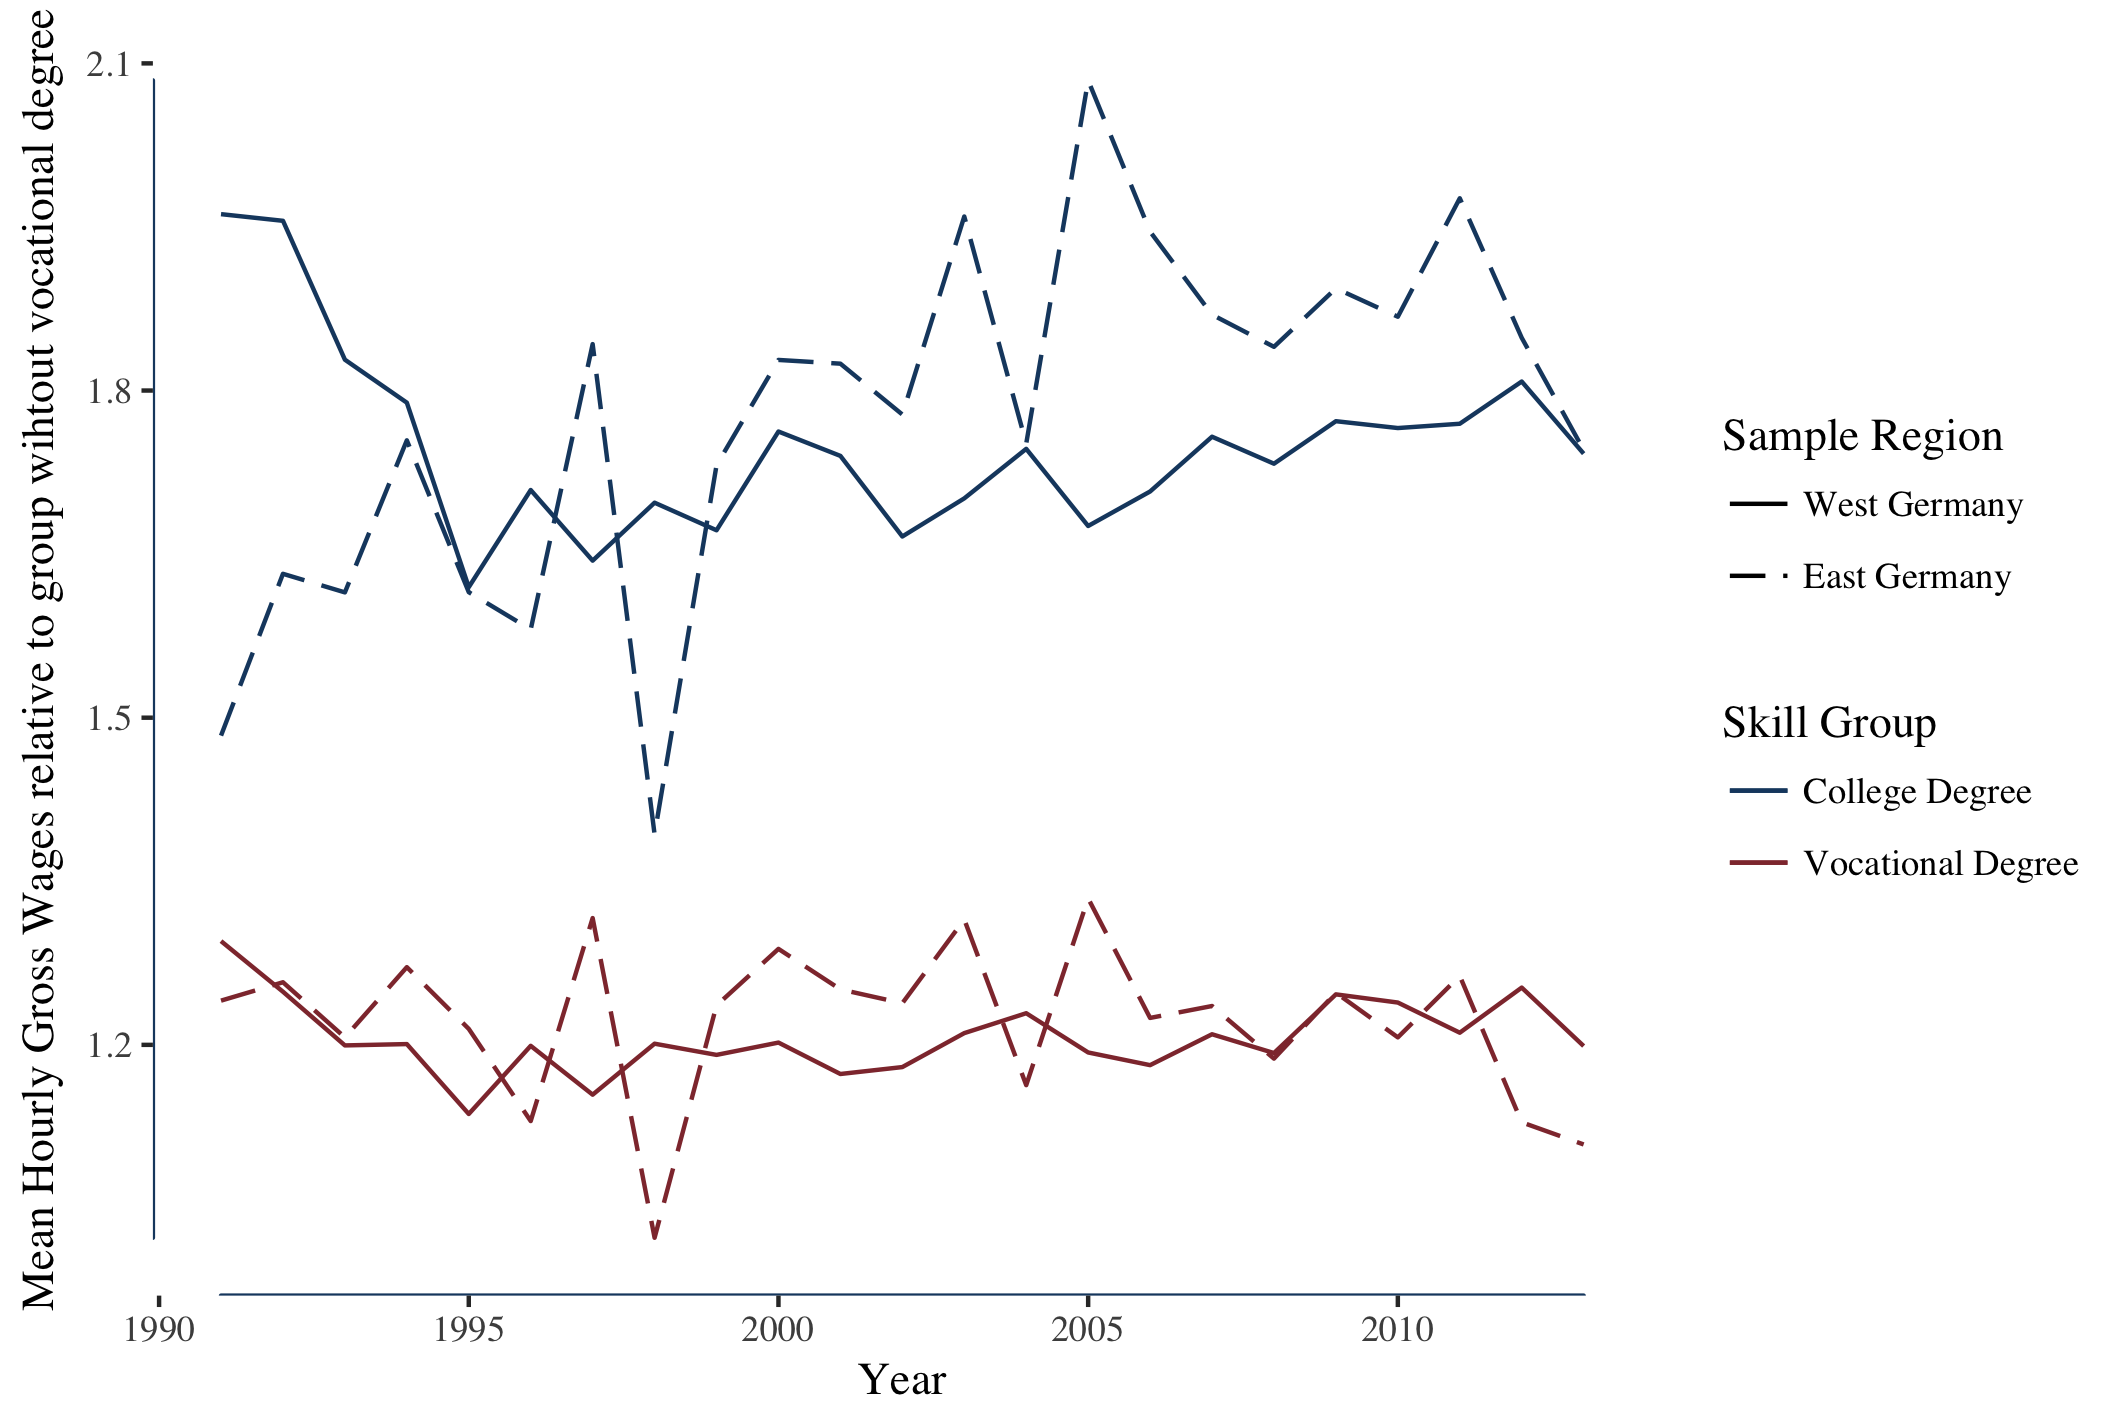
\includegraphics[width=\textwidth]{/Users/Christian/Statistik_Studium/EconProject/Code/Graphics/plotRelHourlyWagesBySkillGroup.png}
    \caption{Relative mean wages across skill groups as multiple of mean wage of workers without vocational degree.}
    \label{fig:RelHourlyWagesBySkillGroup}
\end{figure}

\begin{figure}[!h]
    \centering
    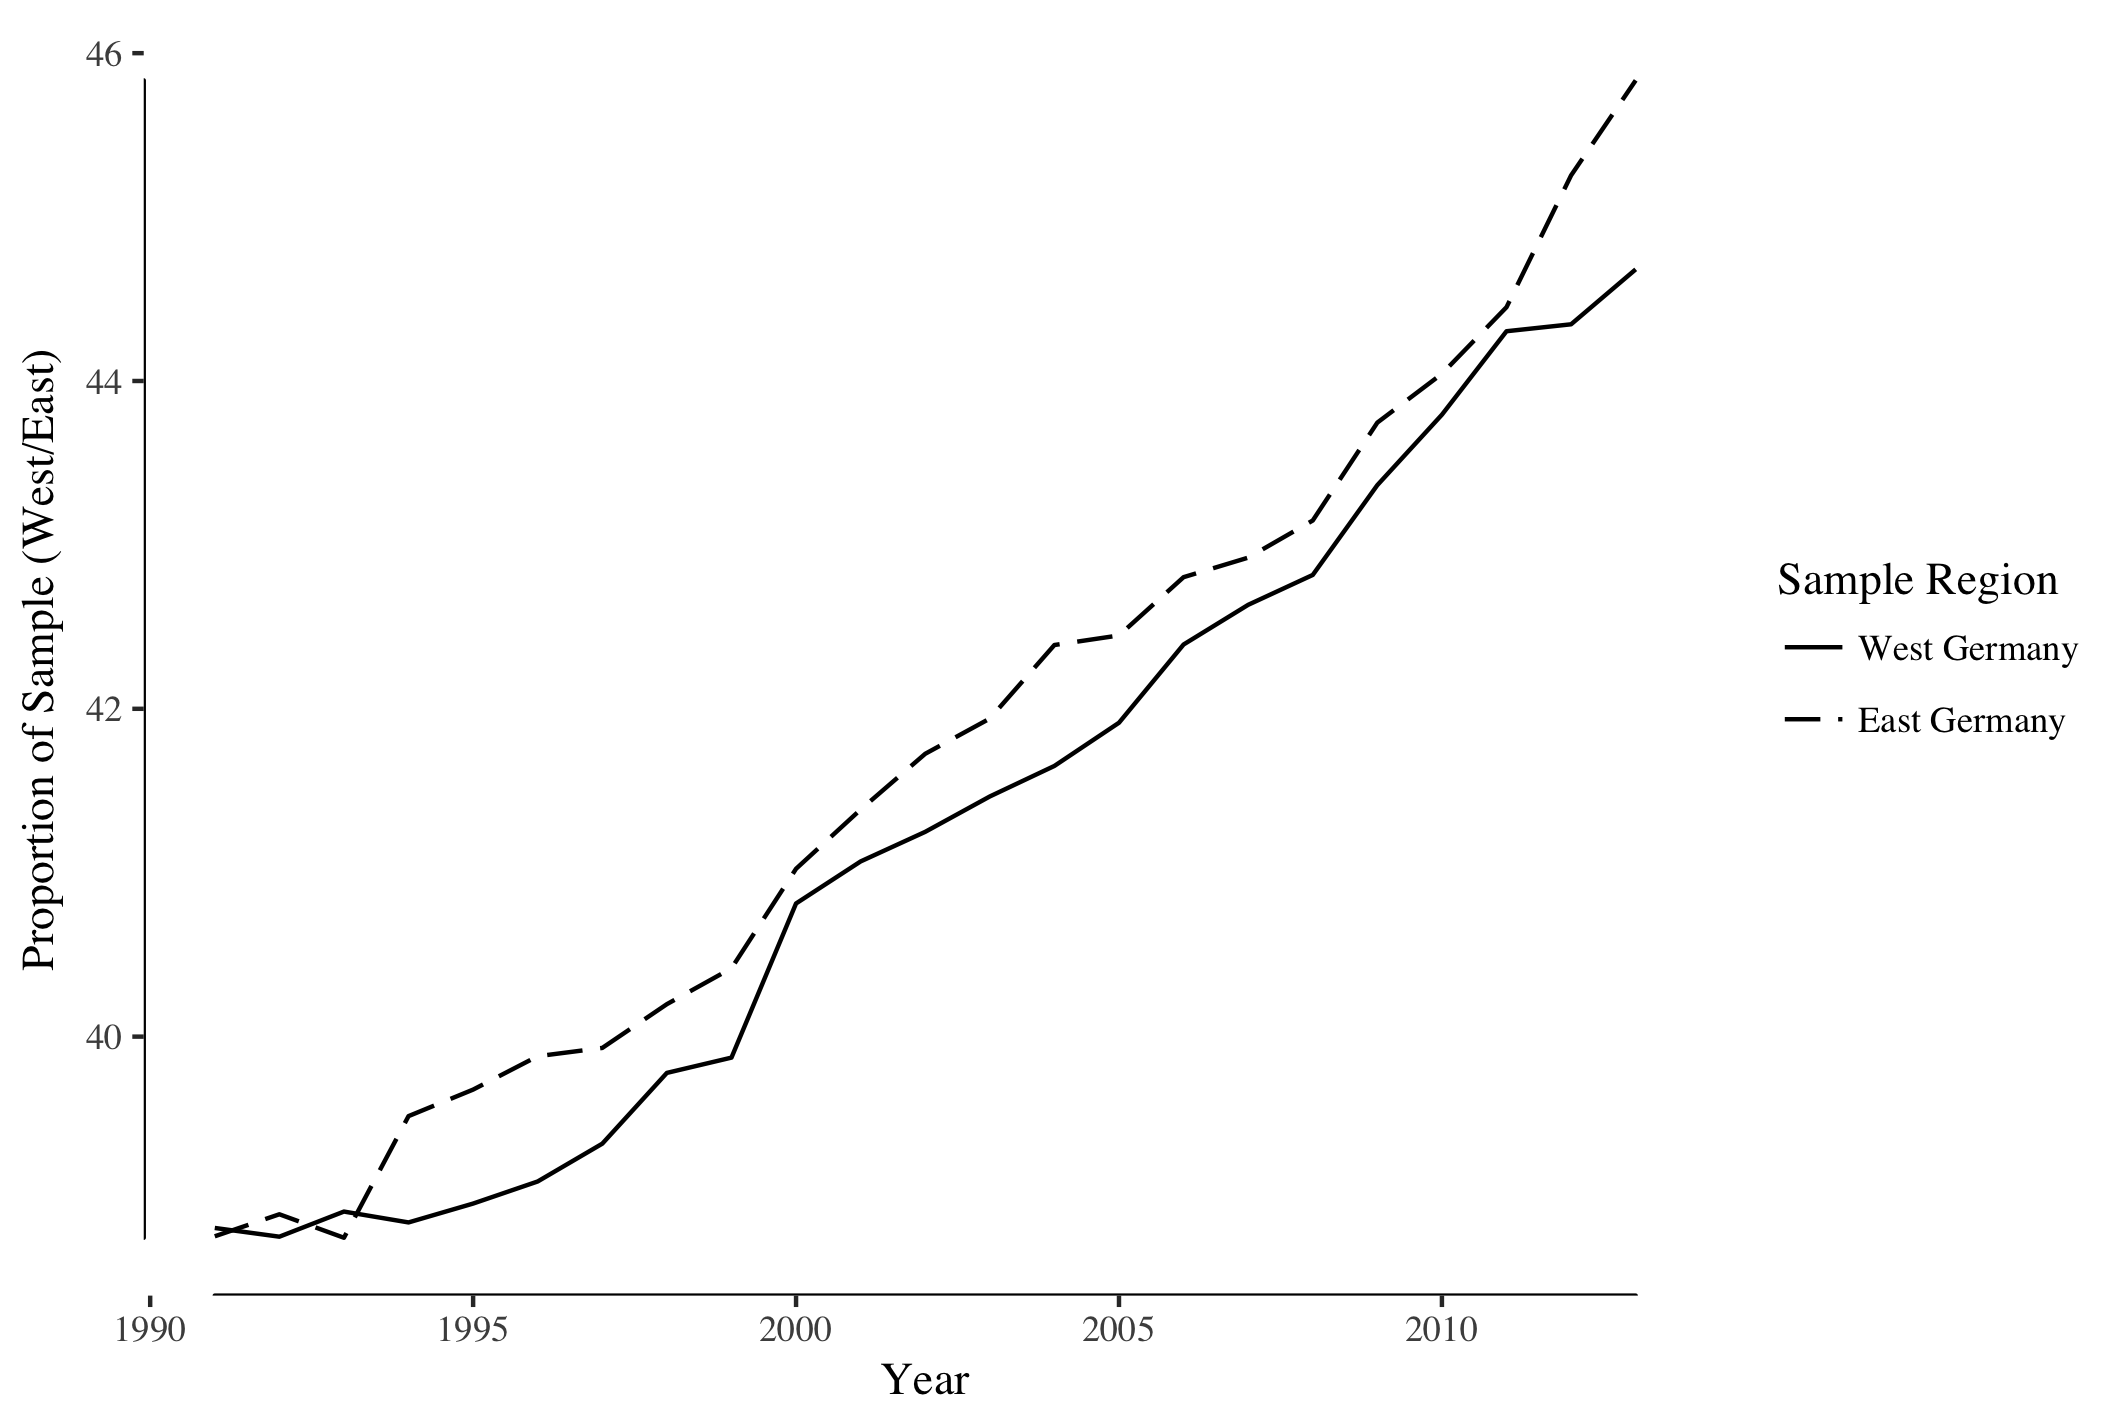
\includegraphics[width=\textwidth]{/Users/Christian/Statistik_Studium/EconProject/Code/Graphics/plotAgeMeans.png}
    \caption{Mean Age by Sample Region}
    \label{fig:AgeMeans}
\end{figure}

\begin{figure}[!h]
    \centering
    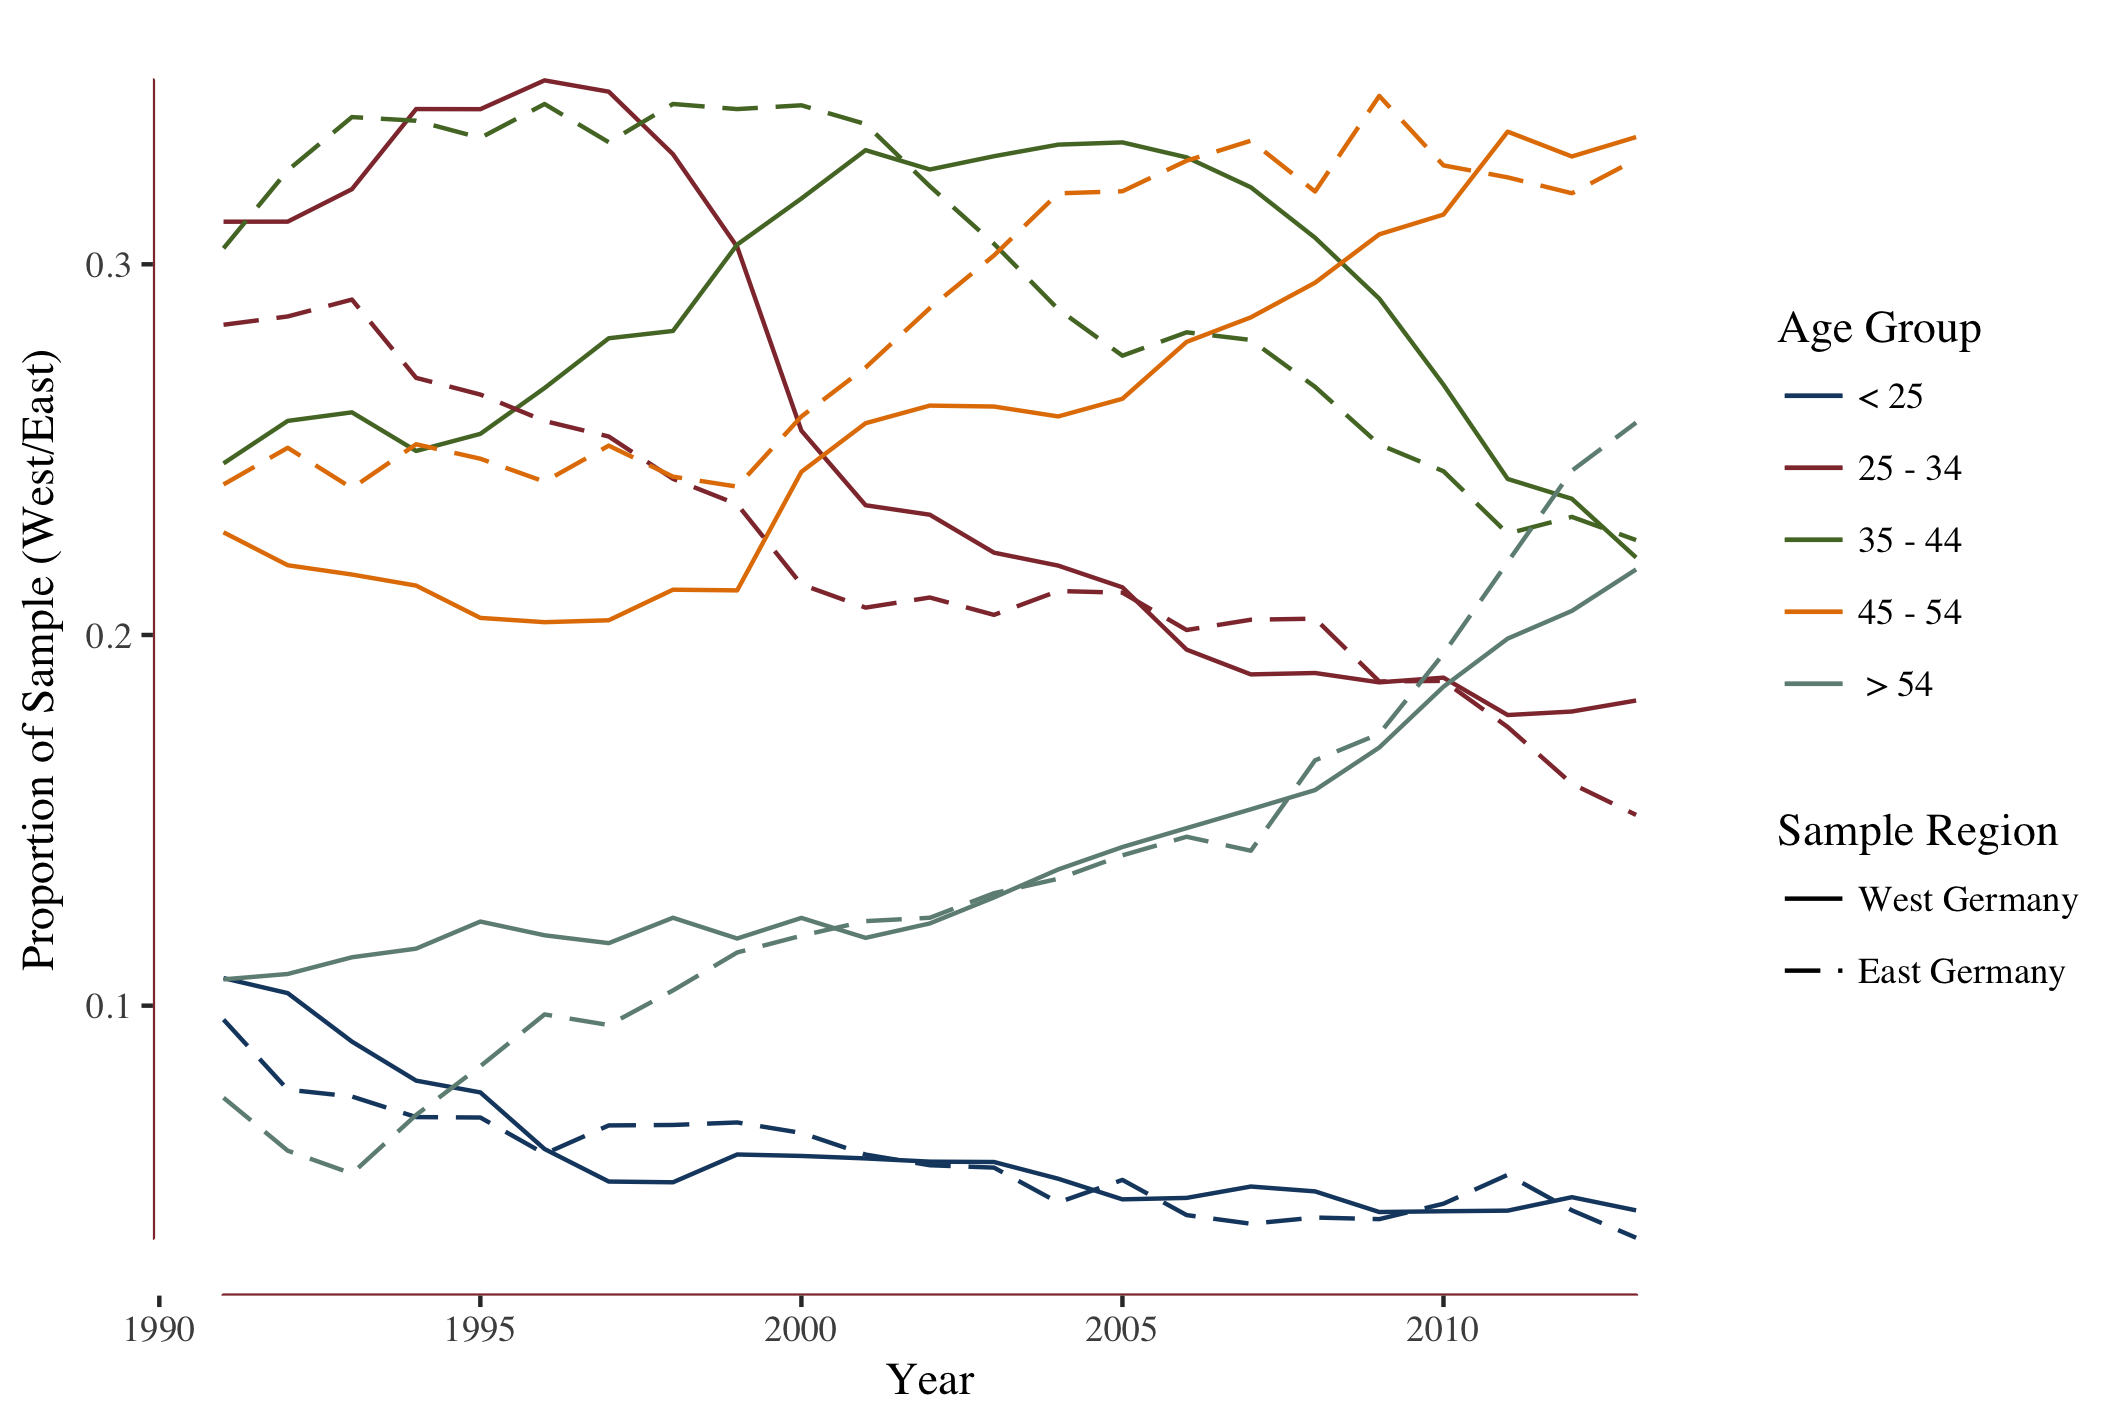
\includegraphics[width=\textwidth]{/Users/Christian/Statistik_Studium/EconProject/Code/Graphics/plotAgeProps.png}
    \caption{Proportion of Age Groups across Sample Regions}
    \label{fig:AgeProps}
\end{figure}

\begin{figure}[!h]
    \centering
    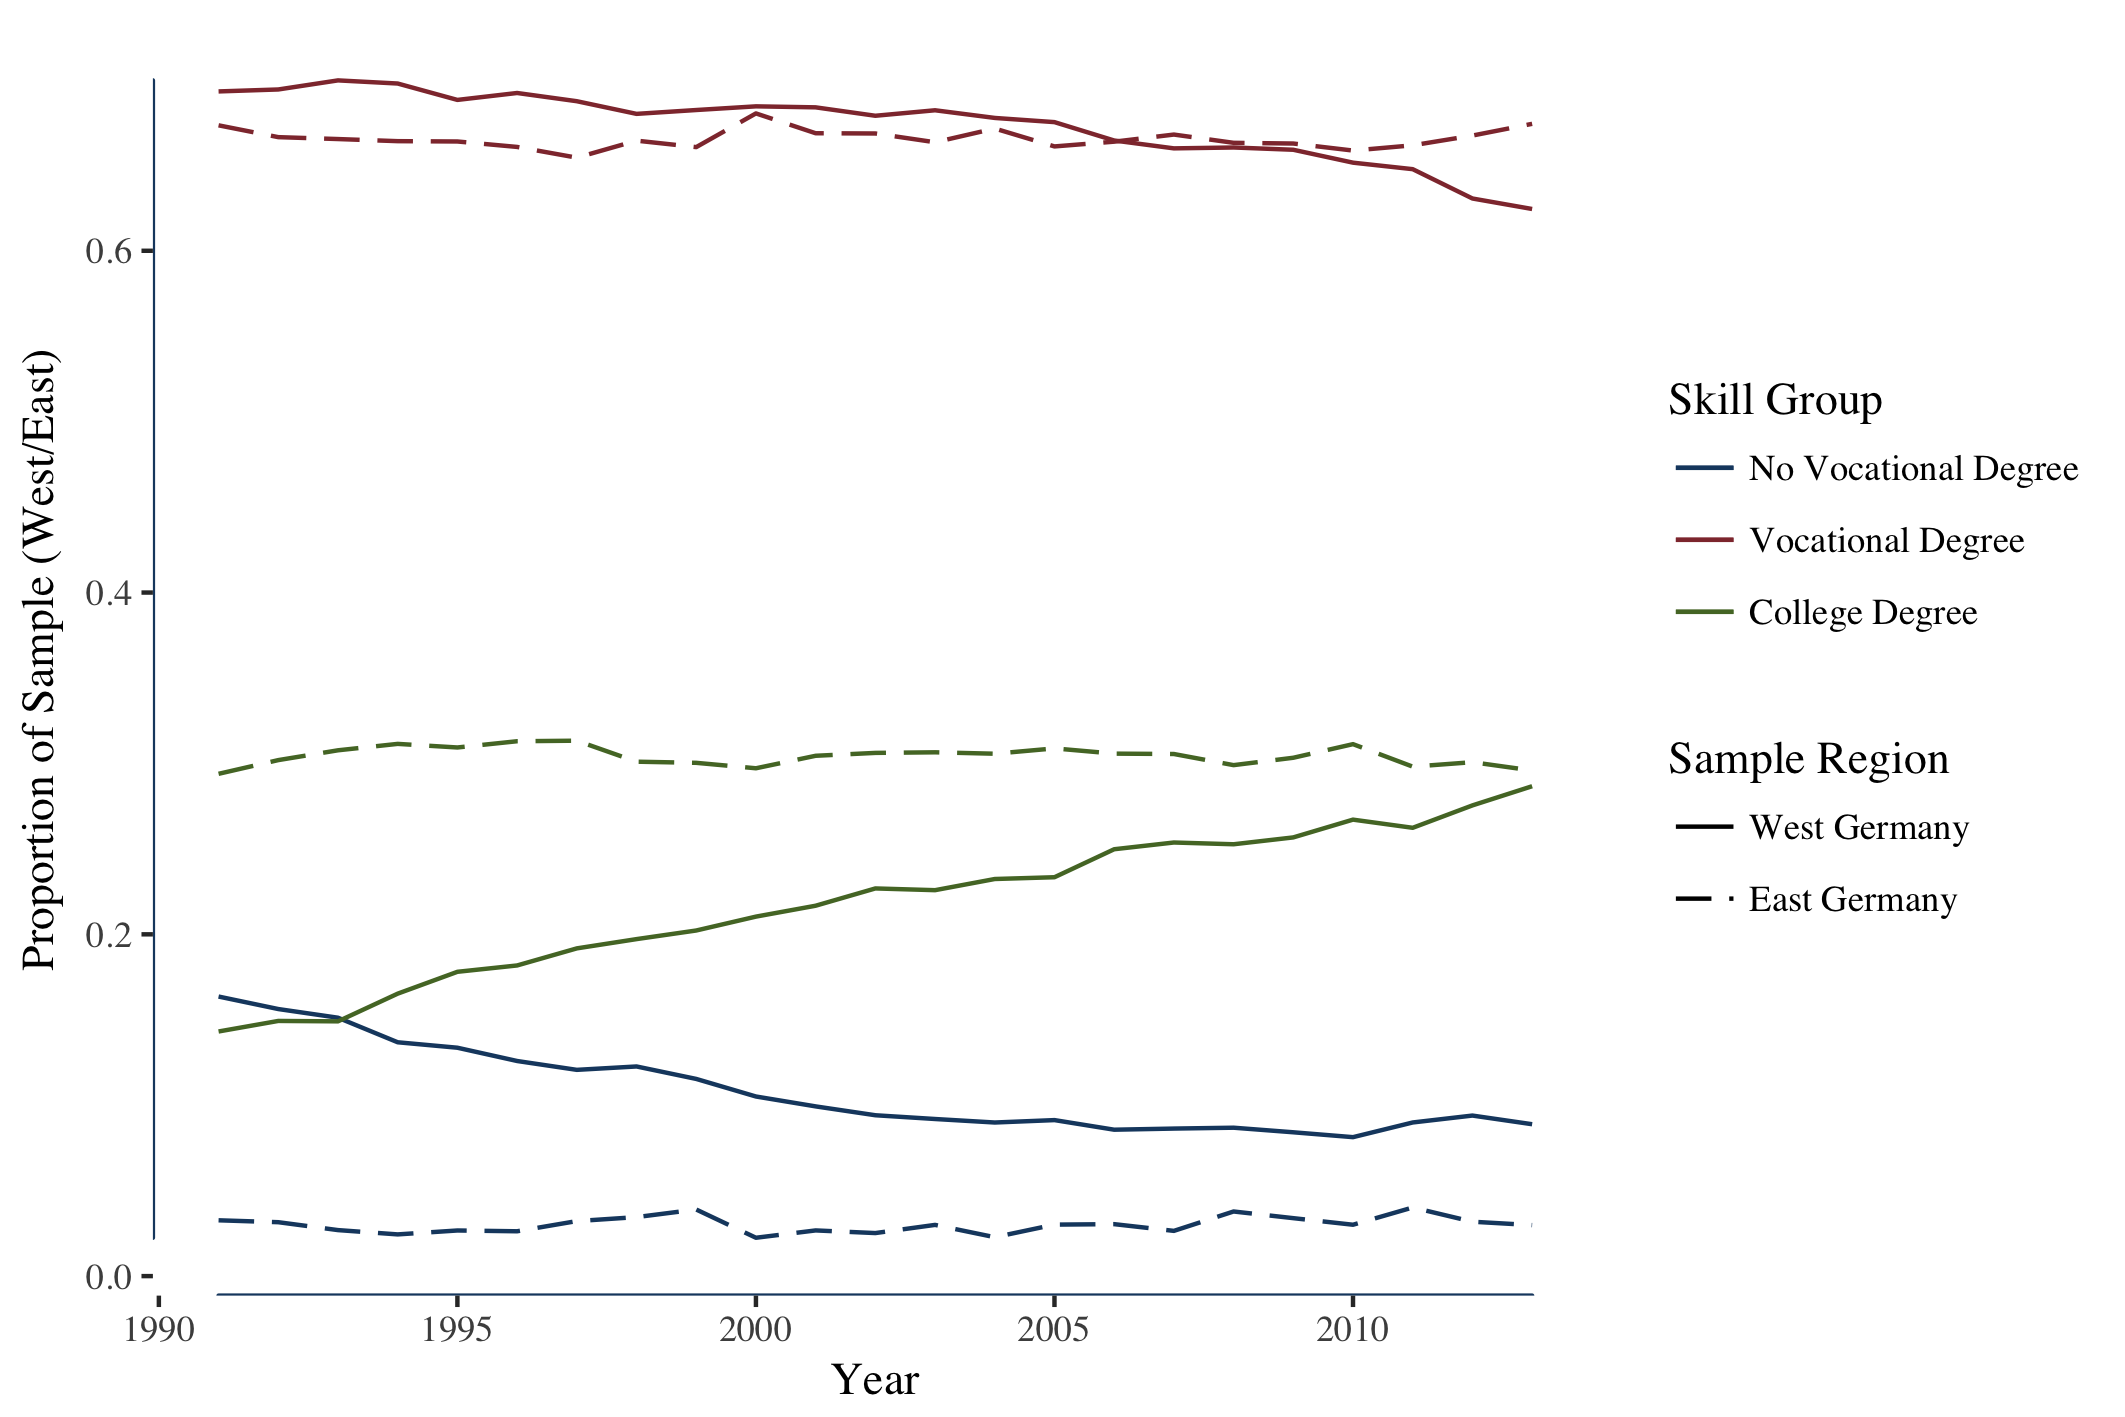
\includegraphics[width=\textwidth]{/Users/Christian/Statistik_Studium/EconProject/Code/Graphics/plotSkillProps.png}
    \caption{Proportion of Skill Groups across Sample Regions}
    \label{fig:SkillProps}
\end{figure}

\begin{figure}[!h]
    \centering
    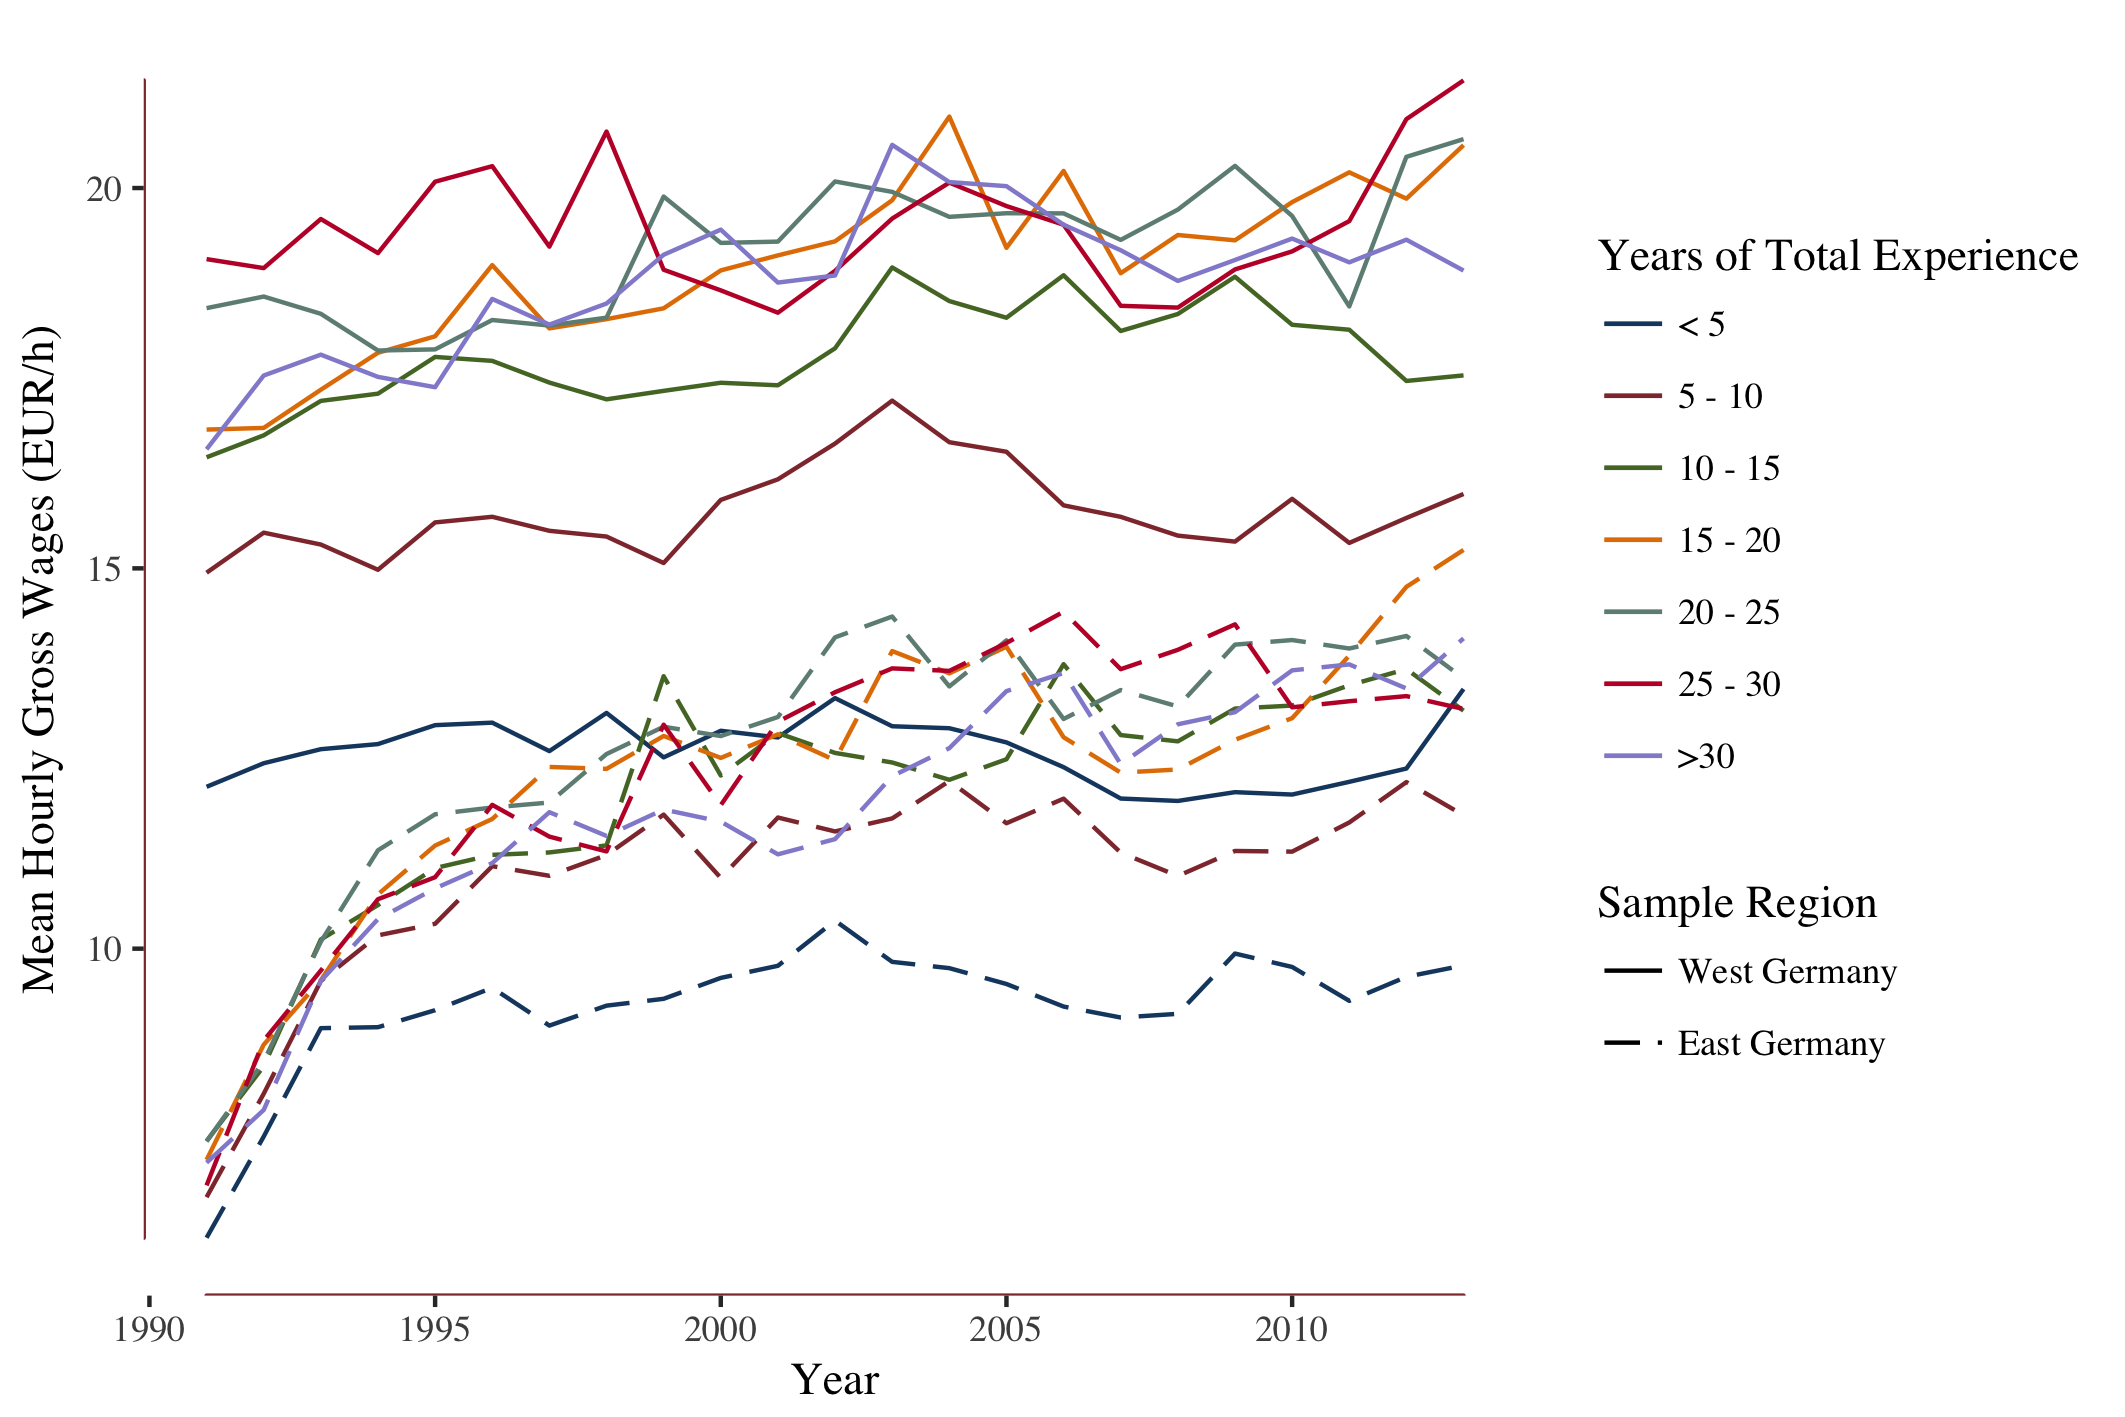
\includegraphics[width=\textwidth]{/Users/Christian/Statistik_Studium/EconProject/Code/Graphics/plotMeanHourlyWagesByExpGroup.png}
    \caption{Average Hourly Wages across Experience Group and Sample Region}
    \label{fig:MeanHourlyWagesByExpGroup}
\end{figure}

\begin{figure}[!h]
    \centering
    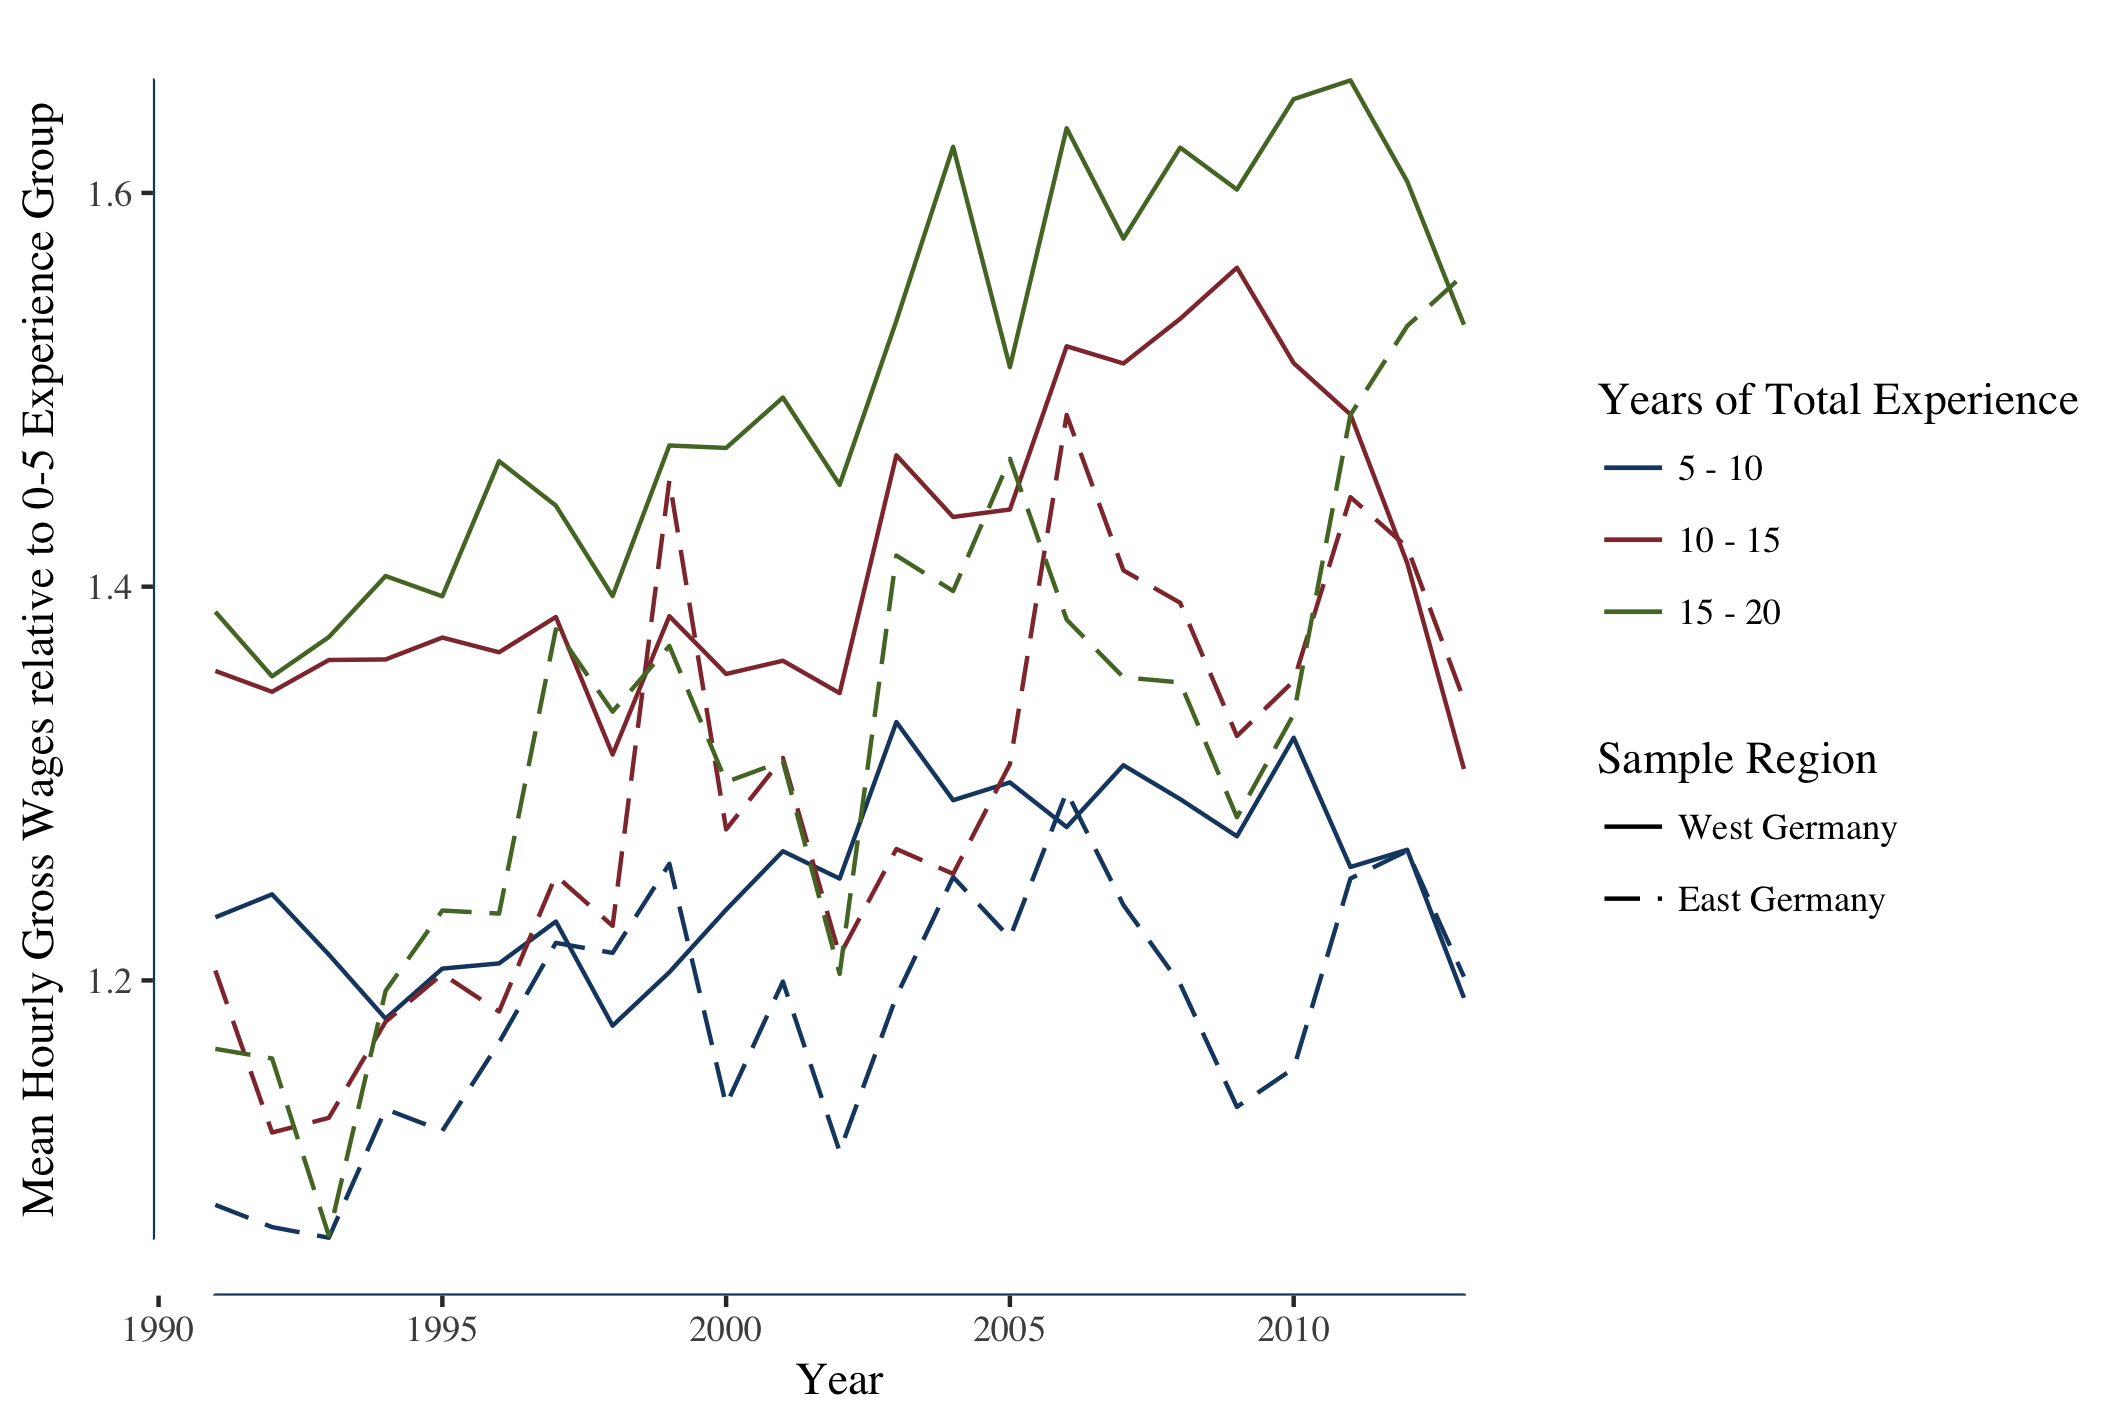
\includegraphics[width=\textwidth]{/Users/Christian/Statistik_Studium/EconProject/Code/Graphics/plotRelHourlyWagesByExpGroup.png}
    \caption{Relative mean wages across selected experience groups as multiple of 0-5 experience group.}
    \label{fig:RelHourlyWagesByExpGroup}
\end{figure}

\begin{figure}[!h]
    \centering
    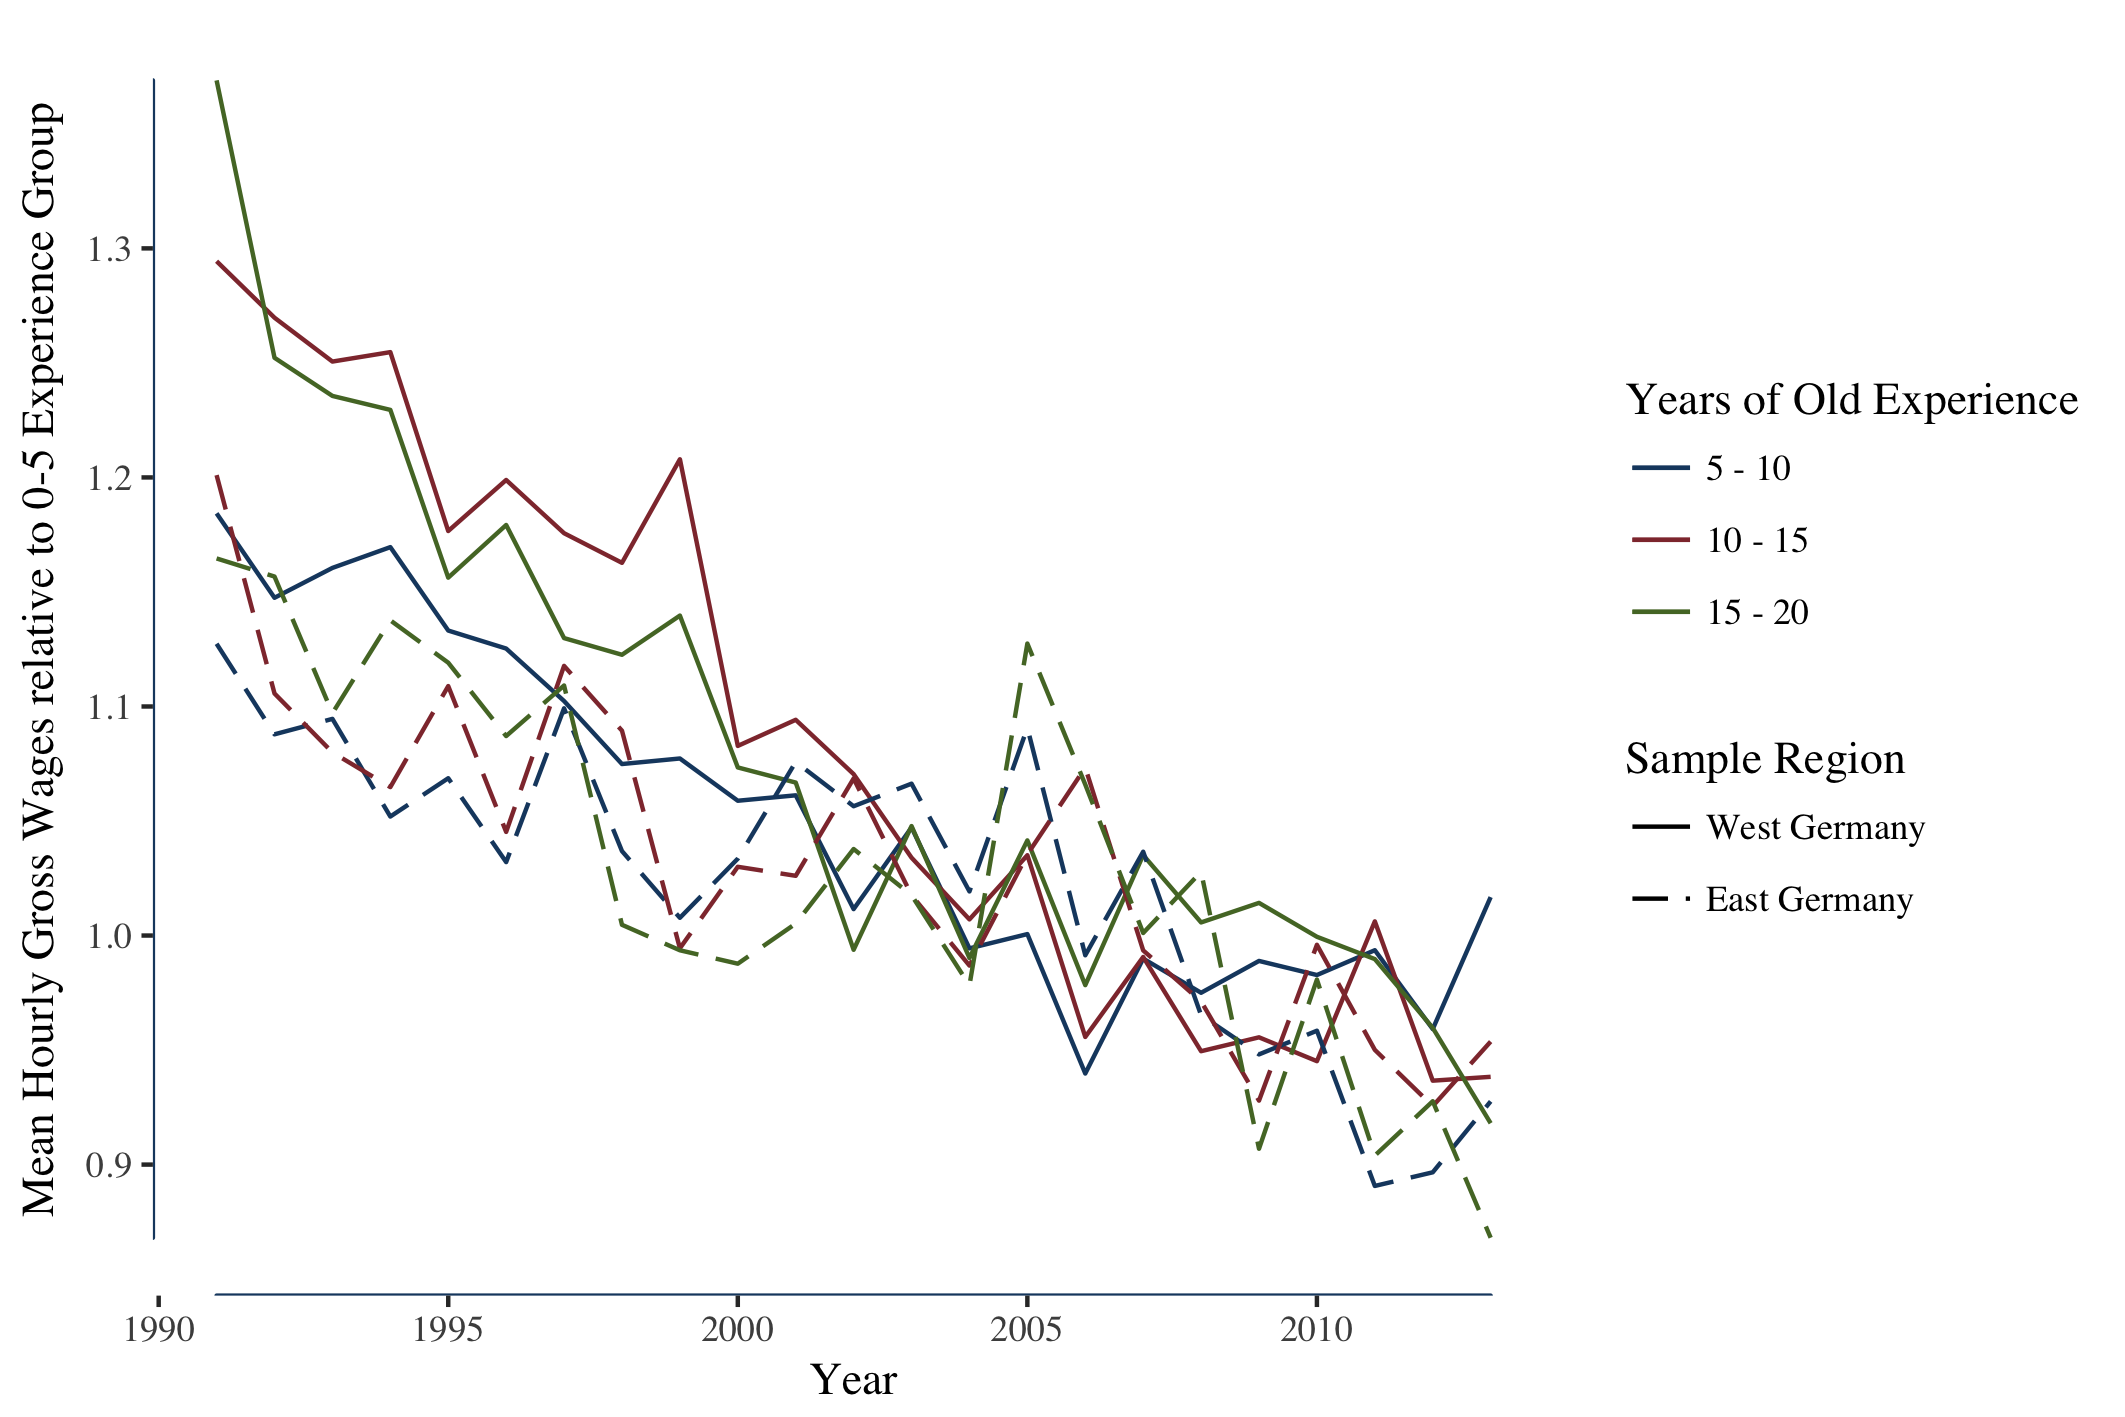
\includegraphics[width=\textwidth]{/Users/Christian/Statistik_Studium/EconProject/Code/Graphics/plotRelHourlyWagesByOldExpGroup.png}
    \caption{Relative mean wages across selected old experience groups as multiple of 0-5 old experience group.}
    \label{fig:RelHourlyWagesByOldExpGroup}
\end{figure}

\begin{figure}[!h]
    \centering
    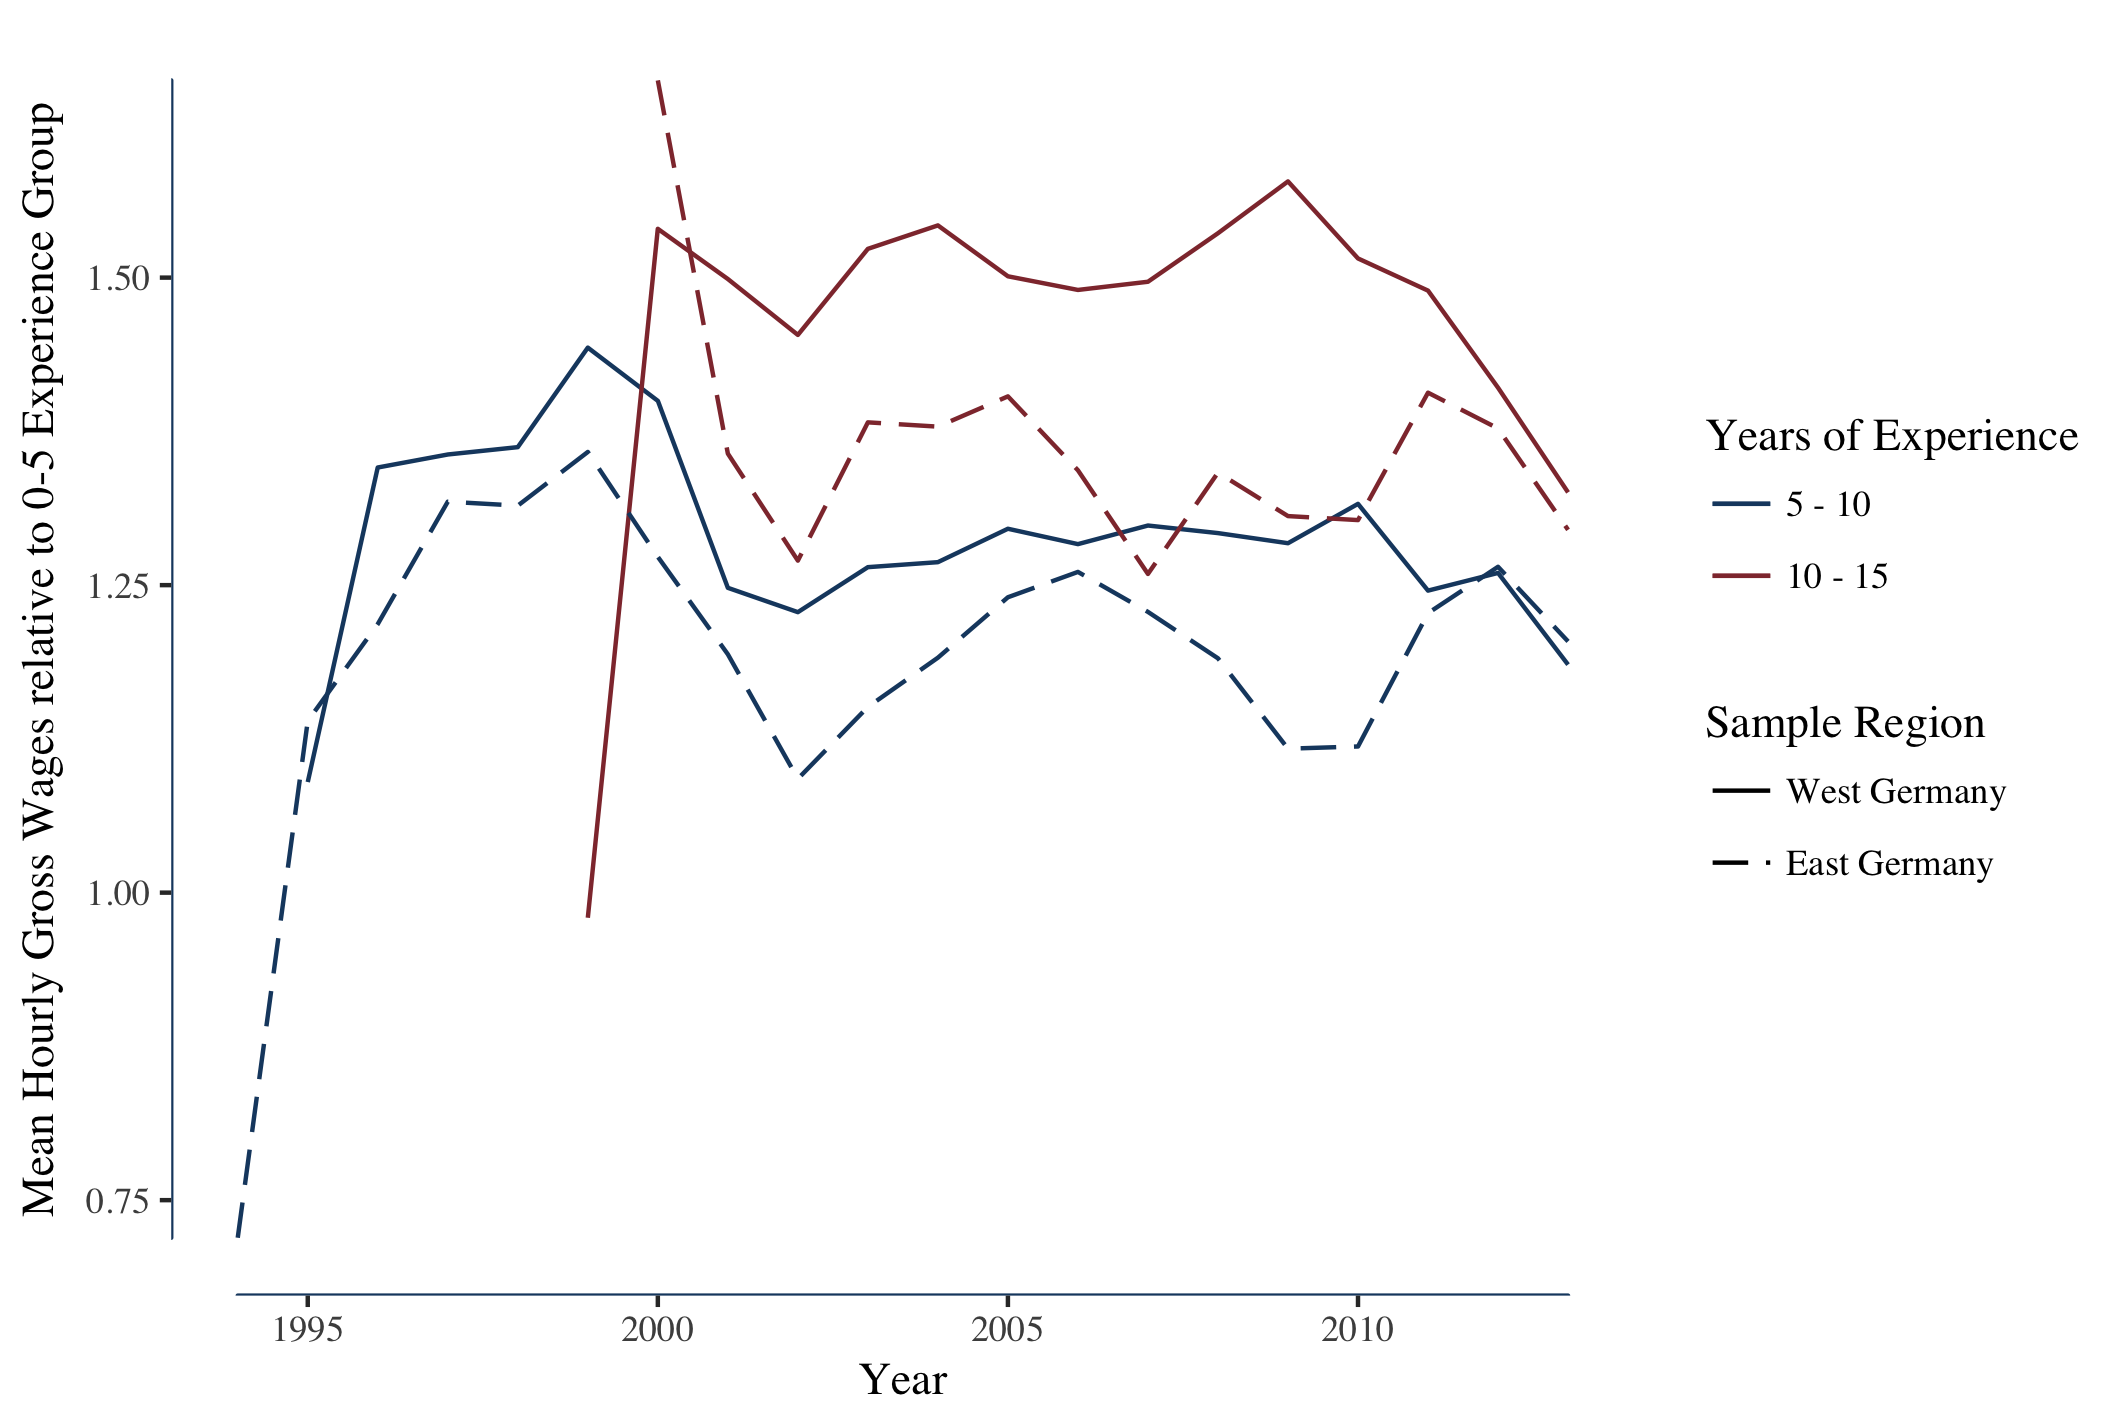
\includegraphics[width=\textwidth]{/Users/Christian/Statistik_Studium/EconProject/Code/Graphics/plotRelHourlyWagesByNewExpGroup.png}
    \caption{Relative mean wages across selected new experience groups as multiple of 0-5 new experience group.}
    \label{fig:RelHourlyWagesByNewExpGroup}
\end{figure}

\end{document}


